\documentclass[
uplatex,
b5paper,
10pt,
%english,
dvipdfmx
]{jsbook}
\usepackage{nruby}
\usepackage{type1cm} % 任意サイズの拡大縮小を可能にする
\usepackage[dvipdfmx]{hyperref}
\usepackage{pxjahyper}
\hypersetup{% hyperrefオプションリスト
 setpagesize=false,
 bookmarksnumbered=true,%
 bookmarksopen=true,%
 colorlinks=true,%
 linkcolor=black,
 urlcolor=black,
 citecolor=red,
}

\usepackage{framed}
\usepackage{wrapfig}
\usepackage{scalefnt}
\usepackage{version,url,here}	% required for `\comment' (yatex added)
\usepackage[dvipdfmx]{graphicx}	% required for `\includegraphics' (yatex added)
\usepackage{natbib,url}
\usepackage{pdfpages}
%\usepackage[varg]{txfonts}
\usepackage{makeidx}
%\usepackage{listings,jlisting}
\usepackage{listings,plistings}
\usepackage{color}
%\usepackage{xcolor}
\lstloadlanguages{[LaTeX]TeX, sh}
\colorlet{lstcolTeX}{green!50!black}
\colorlet{lstcoltext}{black}
\colorlet{lstcolshell}{blue!50!black}

\newcounter{marginparcntbw}[chapter]
\newcommand{\theMarginparcntbw}{$\dagger$\arabic{marginparcntbw}}
\newcommand{\Marginparbw}[2][−10pt]{%
  \stepcounter{marginparcntbw}%
  \textsuperscript{\theMarginparcntbw}%
  \protect\marginpar{\vskip#1\footnotesize%
    \textsuperscript{\theMarginparcntbw}
    {#2}\par}}


\setlength{\fboxsep}{.5zw}
\setlength{\fboxrule}{.6pt}

\begin{comment}
\lstset{basicstyle=\small\ttfamily, keywordstyle={}, commentstyle={},
  columns=flexible, showspaces=false, showstringspaces=false,
  aboveskip=12pt, belowskip=12pt, frame=tb,
  framesep=8pt, framerule=2pt, xleftmargin=10pt,
  xrightmargin=10pt, framexleftmargin=10pt, framexrightmargin=10pt
}
\end{comment}

\lstdefinestyle{shell}{language=sh, rulecolor=\color{lstcolshell!25}}
\lstdefinestyle{TeX}{language=TeX, rulecolor=\color{lstcolTeX!25}}
\lstdefinestyle{text}{language=TeX, rulecolor=\color{lstcoltext!25}}
\begin{comment}
\lstnewenvironment{listing}[1][]
{\lstset{#1}}
{}
\end{comment}


\lstset{% 
language={C++}, 
% backgroundcolor={\color[gray]{.85}},% 
basicstyle={\small},% 
identifierstyle={\small},% 
%commentstyle={\small\ttfamily \color[rgb]{0,0.5,0}},% 
%keywordstyle={\small\bfseries \color[rgb]{0,0,1}},% 
ndkeywordstyle={\small},% 
stringstyle={\small\ttfamily}, 
frame={tb}, 
breaklines=true, 
columns=[l]{fullflexible},% 
numbers=left,% 
xrightmargin=0zw,% 
xleftmargin=3zw,% 
numberstyle={\scriptsize},% 
stepnumber=1, 
numbersep=1zw,% 
morecomment=[l]{//}% 
} 

\begin{comment}
\lstset{
    basicstyle={\ttfamily\footnotesize}, %書体の指定
    keywordstyle={\footnotesize\ttfamily},%
%    frame=tRBl, %フレームの指定
    frame={t}, %フレームの指定
    framerule=1.2pt, %フレームの指定     
%    frame=leftbar, %フレームの指定
    framesep=0pt, %フレームと中身(コード)の間隔
    breaklines=true, %行が長くなった場合の改行
    linewidth=1\textwidth, %フレームの横幅
    xrightmargin=3zw,%
    xleftmargin=3zw,%
    numbers=left,%
    numberstyle={\ttfamily\scriptsize},%
    lineskip=0\baselineskip, %行間の調整
    tabsize=2 %Tabを何文字幅にするかの指定
}
\end{comment}

%\usepackage[format=hang,labelsep=colon,margin=10pt,sc,small]{caption}
\bibpunct[:\,]{(}{)}{,}{a}{}{,}
\definecolor{royalblue}{rgb}{0.0, 0.14, 0.4}
\newcommand{\colorrule}[1]{%
\begingroup\color{#1}\hrule\endgroup%
}%
\newcommand{\Colorrule}[1]{%
\begingroup\color{#1}\rule{1\textwidth}{2.4pt}\endgroup%
}%
\newcommand{\TColorrule}[1]{%
\begingroup\color{#1}\rule[2pt]{1\textwidth}{.6pt}\endgroup%
}%

\usepackage{framed}
\usepackage{color}
\usepackage{dcolumn}
\newcolumntype{d}[1]{D{.}{.}{#1}}
\usepackage{multicol}

\definecolor{lightgray}{rgb}{0.75,0.75,0.75}

\newtheorem{theo}{定理}[section]
\newtheorem{defi}{定義}[section]
\newtheorem{lemm}{補題}[section]

\makeatletter
\renewenvironment{leftbar}{%
%  \def\FrameCommand{\vrule width 3pt \hspace{10pt}}%  デフォルトの線の太さは3pt
  \def\FrameCommand{\vrule width 1pt \hspace{10pt}}% 
  \MakeFramed {\advance\hsize-\width \FrameRestore}}%
 {\endMakeFramed}
\makeatother

\newenvironment{redleftbar}{%
  \def\FrameCommand{\textcolor{red}{\vrule width 1pt} \hspace{10pt}}% 
  \MakeFramed {\advance\hsize-\width \FrameRestore}}%
 {\endMakeFramed}

\newenvironment{lightgrayleftbar}{%
  \def\FrameCommand{\textcolor{lightgray}{\vrule width .5zw} \hspace{10pt}}% 
  \MakeFramed {\advance\hsize-\width \FrameRestore}}%
{\endMakeFramed}


\AtBeginDvi{\special{papersize=\the\paperwidth,\the\paperheight}}

\newcommand{\mini}[2]{%
\setbox0=\hbox{\tt#1}\dp0=4pt%
\setbox1=\hbox{\tiny#2}\ht1=4pt\dp1=7pt%
\leavevmode\vtop{\offinterlineskip\box0\box1}}

\newif\ifVOLONE
\newif\ifVOLTWO
\newif\ifVOLTHREE

\VOLONEfalse
\VOLTWOtrue
\VOLTHREEfalse


% Japanese用の条件マクロ
\newif\ifJapanese
\newif\ifEnglish
%\Japanesefalse
\Japanesetrue   

% English用の条件マクロ
\ifJapanese
\renewcommand{\lstlistlistingname}{プログラム一覧}
\Englishfalse
\else
\Englishtrue
\fi

\newif\ifBLANK
%\BLANKtrue
\BLANKfalse

\newif\ifBIB
%\BIBtrue
\BIBfalse

\newif\ifINDEX
\INDEXtrue
%\INDEXfalse

\newif\ifOUT
%\OUTtrue
\OUTfalse

\newif\ifSHADOW
%\SHADOWtrue
\SHADOWfalse

\newif\ifSchedule
%\Scheduletrue
\Schedulefalse

\newif\ifBook
%\Booktrue
\Bookfalse

\newif\ifPreface
\Prefacetrue
%\Prefacefalse


\newif\ifCHSummary
%\CHSummarytrue
\CHSummaryfalse

\newif\ifPOSTSCRIPT
%\POSTSCRIPTtrue
\POSTSCRIPTfalse

\newif\ifWORKBOOK
\WORKBOOKtrue
%\WORKBOOKfalse


\newif\ifPLAYGAME
%\PLAYGAMEtrue
\PLAYGAMEfalse

\newif\ifVOCAB
%\VOCABtrue
\VOCABfalse

\newif\ifDEVELOPPER
%\DEVELOPPERtrue
\DEVELOPPERfalse

\ifWORKBOOK
\DEVELOPPERfalse
\Prefacetrue
\Booktrue
\CHSummaryfalse
\fi



\newcounter{excount}
\setcounter{excount}{0}
\newcounter{kdcount}
\setcounter{kdcount}{0}
\newcounter{ancount}
\setcounter{ancount}{0}
\newcounter{columncnt}
\setcounter{columncnt}{0}


\ifBook
\newenvironment{toiquestion}{%
\vspace{-1\baselineskip}
\noindent
\refstepcounter{excount}
\begin{quote}%
 \bfseries 
 \hspace{-2zw}問\theexcount\hspace{.7zw}%
}{%
\end{quote}
%\vspace{1.5\baselineskip}
%\vspace{-.5\baselineskip}
}
\else
\newenvironment{toiquestion}{%
\vspace{-1\baselineskip}
\noindent
\refstepcounter{excount}
\begin{quote}%
 \hspace{-2zw}問\theexcount\hspace{.7zw}%
}{%
\end{quote}
%\vspace{1\baselineskip}
%\vspace{-.5\baselineskip}
}
\fi

\newenvironment{toianswer}{%
%\vspace{-2\baselineskip}%
 \begin{quote}
  \parindent=1zw
  \hspace{.6zw}%
}{%
 \end{quote}
}

\setlength\unitlength{1pt}


\ifEnglish
\title{{\LARGE Linguistics}\\\protect\Colorrule{red}\\{\normalsize In very common daily life}}
\author{Hilofumi Yamamoto\\{\small\sc Ph.\,D. in Linguistics}}
\date{Tokyo Institute of Technology}
\else
\title{言語学\\
\vspace{-.5\baselineskip}
\Colorrule{red}\\\normalsize ことば研究史}
\author{山 元 啓 史\\{\small Ph.\,D.\,in Linguistics}}
\date{東京工業大学}
\fi

\makeindex
\begin{document}
\frontmatter
%\maketitle
\thispagestyle{empty}
\setlength\unitlength{1pt}
\begin{picture}(150,70)(70,565)  
% \put(162,182){\fbox{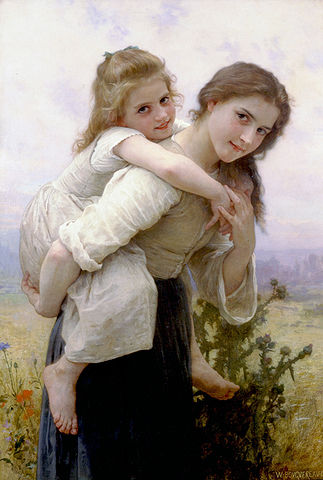
\includegraphics[trim=0 0 0 0,clip,width=0.52\hsize]{William-Bouguereau.jpg}}}
% \put(162,182){\fbox{\includegraphics[trim=0 0 0 0,clip,width=0.51\hsize]{TheDifficultLesson1884.eps}}} 
% \put(172,182){\fbox{\includegraphics[trim=0 0 0 0,clip,width=0.465\hsize]{Sewing1898Edit.jpg}}}
 \put( 0,475){\linethickness{0.4mm}\line(1,0){600}}
 \put( 0,173){\linethickness{0.4mm}\line(1,0){600}}
\ifEnglish
 \put(170,578){\scalefont{2.0}\bfseries Idiomatic Japanese}
 \put(145,555){\scalefont{1.5}\bfseries The Secret of Advanced Japanese}
 \put(230,530){\scalefont{1.8}\bfseries Volume 2}
 \put(210,500){\includegraphics[trim=10 45 10 45, clip, width=12mm]{./edx-logo.eps}}
 \put(245,502){\scalefont{1.5}\itshape\bfseries Tokyo\,Tech\,X}
 \put(100,484){\scalefont{1.5}\bfseries Let's learn Idiomatic Expressions of Japanese}
% \put(210,450){\scalefont{3.0} Workbook}
 \put(160,145){\scalefont{2.0}\bfseries Hilofumi Yamamoto}
 \put(215,130){\itshape\bfseries Ph.\,D.\,in Linguistics}
 \else
 \put(170,578){\scalefont{2.0}\bfseries Idiomatic Japanese}
 \put(145,555){\scalefont{1.5}\bfseries The Secret of Advanced Japanese}
 \put(230,530){\scalefont{1.8}\bfseries Volume 2}
 %\put(210,500){\includegraphics[trim=10 45 10 45, clip, width=12mm]{./edx-logo.eps}}
% \put(245,502){\scalefont{1.5}\itshape\bfseries Tokyo\,Tech\,X}
 \put(100,484){\scalefont{1.5}\bfseries Let's learn Idiomatic Expressions of Japanese}

 \put(160,145){\scalefont{2.0}\bfseries Hilofumi Yamamoto}
% \put(202,162){\scalefont{0.8}\bfseries やま}
% \put(239,162){\scalefont{0.8}\bfseries もと}
% \put(275,162){\scalefont{0.8}\bfseries ひろ}
% \put(312,162){\scalefont{0.8}\bfseries ふみ}
% \put(200,145){\scalefont{2.0}\bfseries 山 元 啓 史}
 \put(215,130){\itshape\bfseries Ph.\,D.\,in Linguistics}
\fi
\end{picture}
\newpage

\ifEnglish
Idiomatic Japanese, Volume 2
\else
日本語らしい日本語: 上級への道 Volume 2
\fi

\setlength\unitlength{1pt}
  \begin{picture}(0,130)(60,100)
%  \put(63,40){\fbox{\includegraphics[trim=0 0 0 0,clip,width=0.3\hsize]{TheDifficultLesson1884.eps}}} 
%  \put(63,40){\fbox{\includegraphics[trim=0 0 0 0,clip,width=0.3\hsize]{Sewing1898Edit.jpg}}}  
%  \put(190,37){
\includegraphics[width=5mm]{./Cc-public_domain_mark_white.eps}}
  
 \ifEnglish
  \put(55,20){\scalefont{1.0} The Difficult Lesson}
  \put(65,06){\scalefont{1.0} 1884 by William-Adolphe Bouguereau (1825--1905)}
  
%File:William-Adolphe Bouguereau (1825-1905) - Sewing (1898) Edit.jpg
  
 \else
  \put(55,20){\scalefont{1.0} The Difficult Lesson}
  \put(65,06){\scalefont{1.0} 1884 by William-Adolphe Bouguereau (1825--1905)}
  
  \fi
  \end{picture}
% https://commons.wikimedia.org/wiki/File:Mary_Lemon_Waller_-_Spring_Voices_royalacademyillu1896roya_0070.jpg
\vfill

Hilofumi Yamamoto, Ph.\,D. in Linguistics, Tokyo Institute of Technology

\textcopyright\,Hilofumi Yamamoto, 2019


\ifPreface
\ifEnglish
\chapter*{Preface}
\else
\chapter*{はじめに}
\fi

\ifEnglish
This is one of the Japanese textbooks by edX MOOCs Tokyo Institute of Technology Online Education Development Room.
There is a knack to studying languages.
You should not stick to the details of it.
It is also necessary to get used to thinking that it does not matter.
No matter how much the structure of the bicycle you study, you will not be able to ride a bicycle.
There are many people who are riding a bicycle with no knowledge of the structure of the bicycle.
Just watching a bicycle will not allow you to ride a bicycle.
Anyway, if you do not ride a bicycle, you will not be able to ride.
Let's try it.

\else

本書はedX MOOCs 東京工業大学オンライン教育開発室による日本語の教科書である。
言語の勉強にはコツがあります。
詳細なところにこだわらないことである。
どうでも良いと考えることに慣れることも必要である。
自転車の構造をいくら勉強しても、自転車には乗れない。
自転車の構造を知らないで自転車に乗っている人はたくさんいる。
自転車を見ているだけでは、自転車に乗れない。
とにかく自転車に乗らなければ、乗れるようにはなれない。
やってみよう。
\fi

\vspace*{1\baselineskip}
\begin{flushright}
 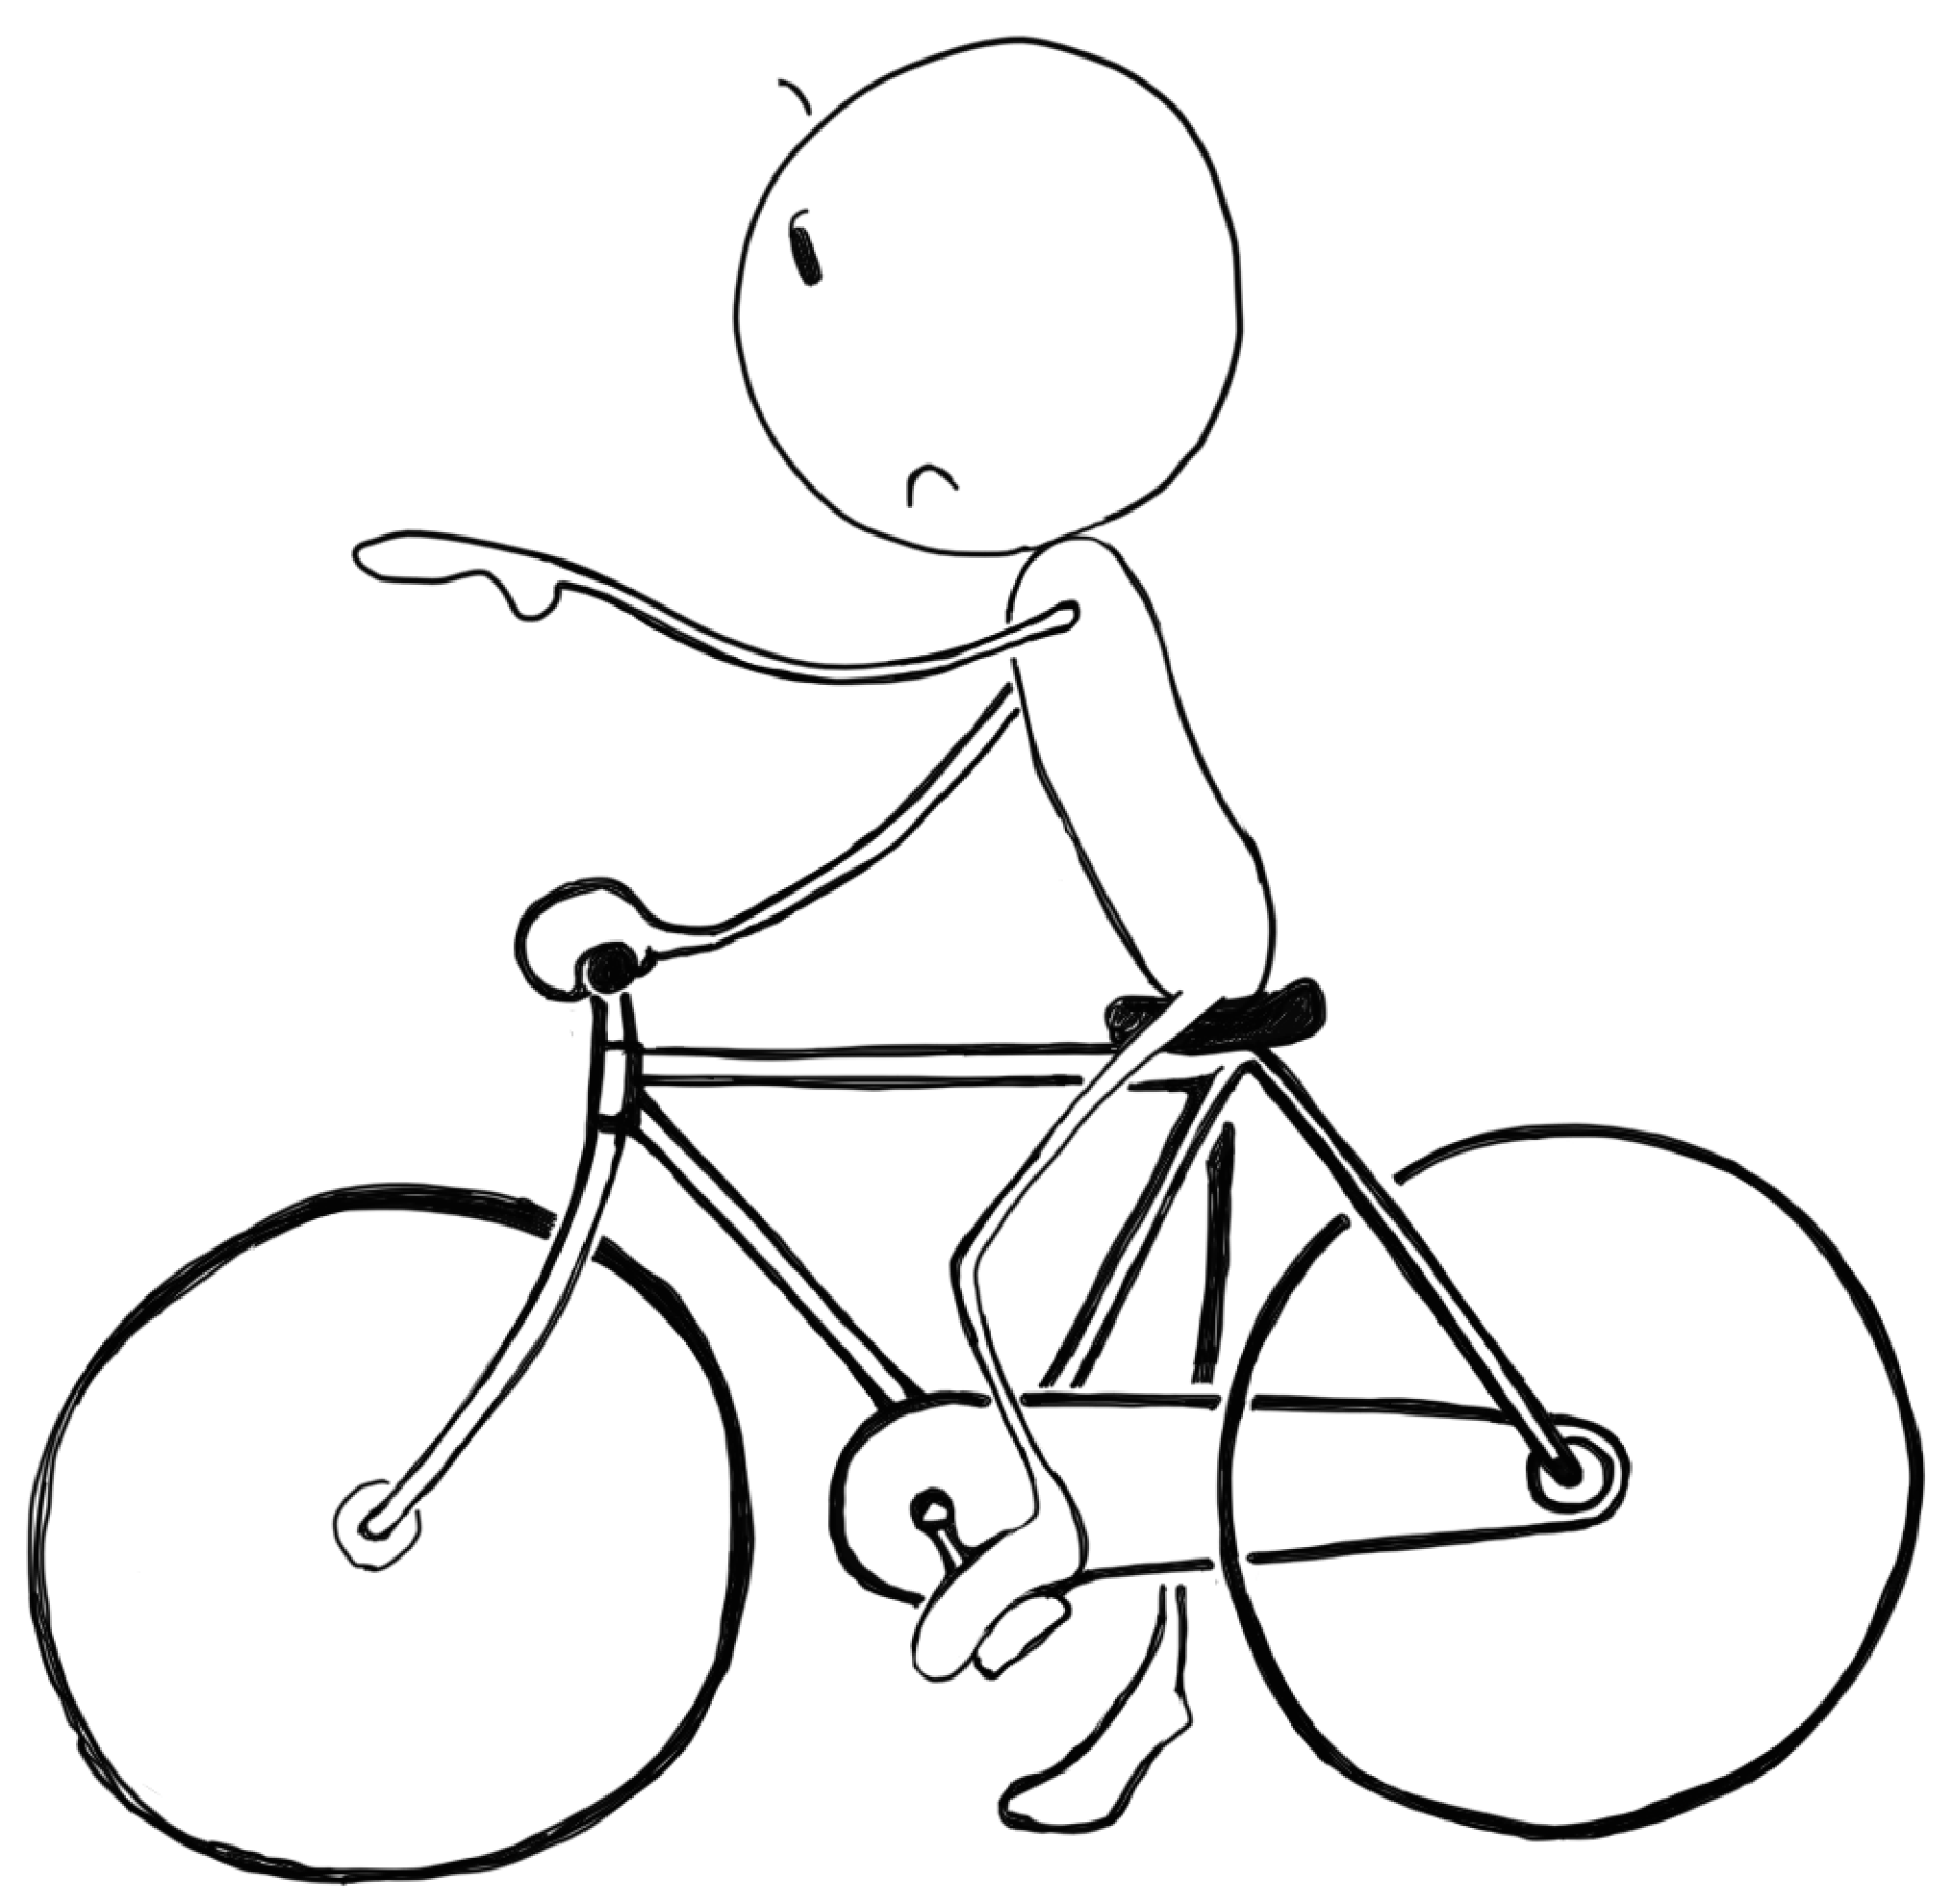
\includegraphics[width=.2\hsize]{bicycle201801.pdf}

 \ifEnglish
 Hilofumi Yamamoto, Ph.\,D.\\
 Professor of Linguistics\\
 Tokyo Institute of Technology\\
 \else
 {\large 山 元 啓 史}\hspace*{3zw}
 
 {\small 東京工業大学教授\hspace*{2zw}}
\fi
\end{flushright}
%\end{document} % for checking the first page.

\setcounter{tocdepth}{0}
\tableofcontents
%\listoffigures
%\listoftables
%\lstlistoflistings
\mainmatter

\ifEnglish
\chapter{Getting Started}
\else
\chapter{さあ、はじめよう}
\fi

\includepdf[pages=22-31, scale=.84, trim=70 80 70 80, clip, offset=0mm -7mm, pagecommand={\thispagestyle{plain}}]{./idiom_compact.pdf}
\label{113010_11Dec18} % U2S1

\ifEnglish
\chapter{Commentary}
\else
\chapter{解説編}
\fi

%\section*{日本語のイディオムと文型: 91 -- 100}
\begin{enumerate}
\setcounter{enumi}{90}

%91
\index{むちゅうになる@夢中になる}
\index{みすごす@見過ごす}
\index{ふくごうどうし@複合動詞}
\index{しまう@しまう}
\item 9時のニュースを見ようと思っていたのに、本に\underline{ A }になって、
      \underline{ B }てしまった。

\begin{itemize}
% \itemsep=-4pt
\item[□] A 夢中; B 見過ごし、忘れ
\item[◆] 「〜に夢中になる」は「夢の中に入って」という意味ではない。〈〜
	  することだけに全部の気持ちが向かってしまう〉という意味。「夢中
	  で〜する」「〜したときは夢中だった」のような使い方がある。
\end{itemize}
\begin{itemize}
% \itemsep=-4pt
\item 仕事に夢中になって、つい家へ帰るのが遅くなってしまった。
\item おもしろい論文のテーマが見つかって、夢中で調べ始めた。
\item 大人も子供もコンピュータゲームに夢中になっている。
\end{itemize}
\begin{itemize}
% \itemsep=-4pt
\item[◆] 「見過ごす」には次の2つの意味がある。上の例は見ていながら、そ
	  のまま見ないふりをしておく、見逃す、見損なう ←見るときが過ぎ
	  る
\end{itemize}
\begin{itemize}
% \itemsep=-4pt
\index{わけ@わけ}
\item いくら自分が忙しいからといって、友達が困っているのを見過ごすわけに
      はいかない。
\item 掲示板には大事なことが書いてあるので、見過ごさないように注意してく
      ださい。
\end{itemize}


%92
\index{ひとがかわったように@人が変わったように}
\index{よう@よう}
\item それまで毎日遊んでいたのに、急に人が\underline{     }ように真面目に勉
      強しはじめた。

\begin{itemize}
% \itemsep=-4pt
\item[□] 変わった
\item[◆] 「56.手のひらを返すように」は人間関係の中で態度が急に悪くなる
	  場合にだけ使うが、「人が変わったように」は〈別の人間になったよ
	  うに〉と、いい方へも、悪い方へも性格が変わった場合、使う。上の
	  例文では、心を入れ換えて、新しい人間になったように、という意味。
\end{itemize}
\begin{itemize}
% \itemsep=-4pt
\item 太郎さんは、このごろ人が変わったように仕事に意欲的だ。
\item 高校時代勉強しなかった娘が、浪人したら、人が変わったように猛勉強を
      始めた。
\end{itemize}
  
%93
\index{いっときも@一時も}
\index{かのうのひょうげん@可能の表現}
\index{なしでは@なしでは}
\index{すごせない@過ごせない}

\item 父はアルコール中毒なので、お酒なしでは一時(いっとき)も\underline{   }ない。

\begin{itemize}
% \itemsep=-4pt
\item[□] 過ごせ
\item[◆] 「過ごす」は〈時間を送る〉〈暮らす〉の意味。
\end{itemize}
\begin{itemize}
% \itemsep=-4pt
\item 楽しい一時(ひととき)を過ごしました。
\item みなさまいかがお過ごしですか。(手紙文)
\item ドイツではブレーメンの友達の家でしばらく過ごした後、ミュンヘンに行
      きました。
\end{itemize}

%94
\index{みられない@見られない}
\index{かのうのひょうげん@可能の表現}
\index{など@など}
\index{おめにかかれない@お目にかかれない}

\item 現代では家族全員そろって食事をする風景など、まず\underline{    }ない。

\begin{itemize}
% \itemsep=-4pt
\item[□] 見られ、お目にかかれ
\item[◆] 「お目にかかる」は〈会う〉の謙譲語で、「お目にかかれない」とい
	   うのは〈会うことができない〉という意味だが、少し批判的な気持
	   ちで、皮肉に〈見ることができない〉という場合に、このような使
	   い方もある。「まず〜ない」はこの場合、〈めったにない〉という
	   意味。
\end{itemize}
\begin{itemize}
% \itemsep=-4pt
\item 近頃、電車の中でお年寄りに席を譲る人など、めったにおめにかかれない。
\end{itemize}

%95
\index{すぎない@過ぎない}
\index{よる@よる}
\item 統計によると、全員そろって食事をする家庭はわずかに8%に\underline{   }。

\begin{itemize}
% \itemsep=-4pt
\item[□]  過ぎない
\item[◆] 「わずか(に)〜に過ぎない」で、その量が思ったより少ないことを言う。
\end{itemize}
\begin{itemize}
% \itemsep=-4pt
\item 最初30人いたのに、最後までクラスに残ったのはわずか5人にすぎない。
\item あの人は日本語が上手ですが、クラスで勉強したのはわずか2週間にすぎ
      ないんですよ。
\end{itemize}

%96
\index{よりほかない@よりほかない}
\index{のに@のに}
\index{し@し}
\index{より@より}
\index{ほか@ほか}
\item 日曜日なのに、雨も降っているし、お金もないし、家で寝るより\underline{   
       }。

\begin{itemize}
% \itemsep=-4pt
\item[□] ほかない
\item[◆] 「ほかない」は〈他に方法がなく、することができるのは〜だけだ〉
	  の意味。
\end{itemize}
\begin{itemize}
% \itemsep=-4pt
\item 冷凍庫が故障してどんどん中のものが解け始めた。これは、どんどん料理
      して、食べるよりほかない。
\item しまった日曜日なのにお金をおろしわすれた。これは、家でじっとしてい
      るほかない。
\end{itemize}

%97
\index{まさか@まさか}
\index{まい@まい}
\item 彼はまさか外国人では\underline{     }。

\begin{itemize}
% \itemsep=-4pt
\item[□]  あるまい
\item[◆] 「まさか〜ではあるまい/〜するまい」で、〈私は〜だとは思わない
	  し、事実〜ではないだろう、しかし、ちょ{}っとその自分の判断が不安
	  だ〉という意味。
\end{itemize}
\begin{itemize}
% \itemsep=-4pt
\item 毎晩帰りが遅いけど、まさか不倫しているんじゃないでしょうね。
\item いくら失恋したといっても、まさか自殺まではするまい。
\end{itemize}

%98
\index{さすが@さすが}
\index{だけ@だけ}
\index{だけあって@だけあって}
\item \underline{   }声楽科の学生だけあって、普段の声もいいですね。

\begin{itemize}
% \itemsep=-4pt
\item[□]  さすが
\item[◆] 「さすが〜だけあって、...」は〈〜であるから、やはり、...〉で、...
	  の部分はpositive(+イメージ)な事柄がくる。「さすが」と一言で、
	  〈すばらしい〉の意味に使われるが、この場合は、前々からすばらし
	  い能力の人だとはわかっていたが、やっぱりすばらしい能力だと、再
	  確認した、という意味で誉めている。
\end{itemize}
\begin{itemize}
% \itemsep=-4pt
\item (いつもカラオケが上手な人の歌の後)「うまいね。さすがだね。」
\item 「さすが山田さんだけあって、難しい歌が上手だね。」
\end{itemize}

%99
\index{べき@べき}
\index{つくす@尽くす}
\item あなたが悪いのだから、あなたが謝る\underline{    }と思う。

\begin{itemize}
% \itemsep=-4pt
\item[□]  べき、のが当然だ
\item[◆] 「べき」は「当然〜しなければならない」の意味。
\end{itemize}
\begin{itemize}
% \itemsep=-4pt
\item そんなにすぐにあきらめないで。自分のベストを尽くすべきだと思うわよ。
\item 国は安心して老後が暮らせるように、福祉を充実させるべきだ。
\end{itemize}

%100
\index{おろか@おろか}
\index{いくら@いくら}
\index{ても@ても}
\index{さえ@さえ}
\index{めいれいのひょうげん@命令の表現}
\item 1000円は\underline{ A }、10円玉\underline{ B }もないのだ
      から、いくら\underline{ C }と言われても返せない。

\begin{itemize}
% \itemsep=-4pt
\item[□]  A おろか、もちろん; B さえ; C 返せ
\item[◆] 「おろか」 さえも→51 いくら〜ても→11
\end{itemize}
\begin{itemize}
% \itemsep=-4pt
\item その町は死んだように静かで、人はおろか、犬一ぴきさえいなかった。
\item コンピュータはおろかワープロさえさわったことがない。
\end{itemize}
\end{enumerate}
%end of file


%\section*{日本語のイディオムと文型: 101 -- 110}
\begin{enumerate}
\setcounter{enumi}{100}

%101
\index{ようにも@ようにも}
\index{よう@よう}
\index{かのうのひょうげん@可能の表現}
\index{こそあど@こそあど}
\index{こんなに〜では@こんなに〜では}
\item こんなに激しい雪では、出かけようにも\underline{   }。

\begin{itemize}
% \itemsep=-4pt
\item[□] 出かけられない。
\item[◆] 「〜(よ)うにも、....られない。」は「そうしようと思っ
	  ても、何かの事情でそれができない」という意味。このよう
	  に、いつも文末は否定の可能形となる。
\end{itemize}

\begin{itemize}
% \itemsep=-4pt
\item 値段が高すぎて買おうにも買えない。
\item 頭が痛くて、起きようにも起きられない。
\item あまりにも疲れすぎていたので仕事をしようにもできなかった。
\item こんな難しい問題では答えようにも答えられない。
\item 写真が壁にはってあって、彼を忘れようにも忘れられない。  
\item となりの部屋の人たちがあまりにもうるさかったので、寝ようにも寝られ
      なかった。
\item さっき、調理師が料理中にくしゃみをしたのを見たので、この料
      理は食べようにも食べられない。
\end{itemize}

%102
\index{たところで@たところで}
\index{ところ@ところ}
\index{こそあど@こそあど}
\index{やりもらい@やりもらい}
\index{わけ@わけ}
\item あんな社長に文句を言った\underline{   }で、聞いてくれるわけがない。
\begin{itemize}
% \itemsep=-4pt
\item[□] ところ
\item[◆] 「〜たところで、....ない。」は「〜ても」と同じような意
	  味で「たとえ〜が実現したとしても、....ない。」いつも文
	  末は否定的な意味が来る。
\end{itemize}

\begin{itemize}
% \itemsep=-4pt
\item どんなに本をたくさん買ったところで、読まなければなんにもならない。
\item 今から急いだところで、もう遅いでしょう。
\item いまさらレポートを提出したところで、いい点数は取れないはずだ。
\item この会社に電話をかけたところで、社長に会えないだろう。
\item 怒っている妻に正しいことを言ったところで聞いてくれるわけがない。
\item もうこれ以上話し合ったところでむだだ。
\item 政府が景気の底入れを宣言したところで、国民はそれを信じない。
\item 今さら嘆いてみたところで始まらない。
\item お父さんに車を買うお金を頼んだところで、くれるわけがないと思う。
\item 悪い商品なので、いくら広告したところで、なかなか売れなかった。
\item いくら働いてみたところで、こう物価が高くては、生活は楽にはなりませ
      ん。
\end{itemize}

%103
\index{きり@きり}
\item 手紙を一通よこした\underline{  }、何の音沙汰もない。
\begin{itemize}
% \itemsep=-4pt
\item[□] きり
\item[◆] 「〜たきり、....。」「〜の行動がそれで最後になった。その後は何
	  も行動や状況の 変化がない。「きり」は句切りの「きり」で、これ
	  が最後という意味。
\end{itemize}

\begin{itemize}
% \itemsep=-4pt
\item 外国へ行ったきり、連絡がない。
\item 彼は大切な本を借りていったきり返さない。
\item 三年くらい前、彼とあったきり、会っていない。
\item 彼は卒業したきり、学校へ一度も来ない。
\item 2年前にふるさとにいる友だちを見たきり、何の音沙汰もない。
\item あれっきり彼に会わない。
\item 先月お酒を飲んだきり、今まで一度も飲んでいない。
\item あの人は倒れたきり、起き上がらなかった。
\item ずっと前に離婚したきり、あとはひとり暮しです。
\end{itemize}

%104
\index{させておく@〜させておく}
\index{しえき@使役}
\index{たどうしだいようしえき@他動詞代用使役}
\index{おく@おく}
\index{もったいない@もったいない}
\item この部屋を遊ばせて\underline{  }のはもったいない。

\begin{itemize}
% \itemsep=-4pt
\item[□] おく
\item[◆] 「〜ておく」には「今の状態をそのままにして保つ」という意味と、
	  「後のために今準備として何かをする」という意味とある。遊ばせて
	  おく、というのは「何にも利用しないで、役に立っていない状態に保
	  つ」という意味。
\end{itemize}

\begin{itemize}
% \itemsep=-4pt
\item あの体育館を遊ばせておくのはもったいない。
\item 空いている部屋を学生達に自由に使わせておくのが合理的だと思う。
\item その人を待たせておきなさい。
\item 彼女の好きなようにさせておけ。
\item まだ時間があるから、彼をそのまま眠らせておいてもいいでしょう。
\item 結論を出す前にみなによく考えさせておいた方がいいと思う。
\item 出発するまで時間があるので、子供たちを遊ばせておきましょう。
\item こんなおいしそうなお菓子を食べさせないでおくのは、精神衛生に良くな
      い。
\end{itemize}

%105
\index{ただけに@ただけに}
\index{だけ@だけ}
\index{じはつ@自発}
\item 明治生まれの画家は、彼一人であった\underline{    }、彼の死は大いに悔や
      まれる。
\begin{itemize}
% \itemsep=-4pt
\item[□] だけに
\item[◆] 「〜だけに、...」というのは、〜という事実がなければ、それほど
	  でもないの だが、〜という事実があると、一層よけいに...だ、
	  という表現。
\end{itemize}

\begin{itemize}
% \itemsep=-4pt
\item とってもステキなコンサートであっただけに、おこづかいを全部はたいて
      でも、もう1回見に行きたい。
\item もうすこしで捕まえるところであっただけに、逃げられてしまって残念で
      した。
\item あともう少し頑張れば山頂に着くところであっただけに、やめてしまって
      残念だ。
\item この陶磁器は一つしかないものだけに、大切に取り扱うべきだ。
\item 期待していなかっただけに、喜びも大きい。
\item あの横綱は全勝するところであっただけに、昨日の一敗は残念です。
\item 日本のワールドカップにかけた期待が大きかっただけに、失望も大きかっ
      た。
\item 一生懸命努力していただけに、試験に落ちたのは残念だ。
\end{itemize}

%106
\index{させてしまう@させてしまう}
\index{しえき@使役}
\index{しまう@しまう}
\item 私の不注意で、子どもに大怪我を\underline{    }しまった。
\begin{itemize}
% \itemsep=-4pt
 \item[□] させて
 \item[◆] 使役形について復習しておこう。「先生が学生に答えを言わせた。」
	   というような、他の人に命じてさせる、という使役表現の他に、
	   「とても行きたがったので、ロックコンサートに行かせました。」
	   のように許可の表現がある。ここの例は、命令でも、許可でもない。
	   相手に自分の責任で不利益を引き起こした時に使う使役表現は、自
	   分の責任を認めて、詫びる気持ちがある。そのため、これは、目上
	   の人について話すときも使える。
\end{itemize}

\begin{itemize}
% \itemsep=-4pt
\item 先生をお待たせするといけませんから、私は早く行きます。
\item 待たせてしまってごめんね。むだな時間を使わせてしまってすみませんで
      した。
\item 「散財させてしまって申し訳ございませんでした。」「いいえ」
\item 課長の経営能力の欠如のために、計画をむだぼねに終わらせてしまった。
\item パイロットの不注意で、飛行機を墜落させてしまった。
\item 私が時間を守らなかったために、みんなを待たせてしまった。
\item いつまでも泣いて、友だちを困らせてしまった。
\item タイに旅行したとき、タイの友だちにお金をたくさん使わせてしまった。
\item 論文がなかなか書けなくて、先生を困らせてしまった。
\end{itemize}

%107
\index{にもかかわらず@にもかかわらず}
\item 彼は風邪をひいたにも\underline{     }、マラソン大会で優勝した。
\begin{itemize}
% \itemsep=-4pt
 \item[□] かかわらず
 \item[◆] 「〜にもかかわらず、....する」「〜のに」と同じ文脈で使えるが、
	   「のに」がくだけた会話文で使うのに対して、「にもかかわらず」
	   は硬い表現で、書き言葉で通常は使う。また、「のに」は主観的な
	   感じがするが、「にもかかわらず」は客観的な表現である。

	   「のにも関わらず」のように「の」を入れても使う。「調べた(の)
	   にもかかわらず」「親切(なの)にも関わらず」「寒い(の)にも
	   かかわらず」「病気(なの)にもかかわらず」
\end{itemize}

\begin{itemize}
% \itemsep=-4pt
\item 失敗したにもかかわらず、一生懸命やっている。
\item 度々注意したにもかかわらず、失敗した。
\item 彼は明日が試験であるにもかかわらず、遊んでいる。
\item 彼は体の具合が悪いのにもかかわらず、試合に参加するそうだ。
\item 足を折ったにもかかわらず、うちまで歩いて帰りました。
\item クーデターがあったにもかかわらず、レポーターは、まだ仕事をやってい
      る。
\item 政府が不景気から抜け出すために多くの措置をとっているのにもかかわら
      ず、景気は低迷を続けている。
\item 二人はお互いに愛しているにもかかわらず、父母の反対で結婚できません。
\item 試験があるにもかかわらず、彼女はマラソン大会に出場すると決心した。
\item 雨が降っているにもかかわらず、傘もささずに出て行った。
\item 日曜日にもかかわらず、出勤だ。
\item 資本が少ないにもかかわらず、彼の会社は成功した。
\end{itemize}

%108
\index{なら@なら}
\index{から@から}
\index{てから@てから}
\index{めいれいのひょうげん@命令の表現}
\item 病院に見舞いに行く\underline{    }、もう少し元気になってからに
      しなさい。

\begin{itemize}
% \itemsep=-4pt
\item[□] なら
\item[◆] 仮定の表現で、「Pを実現できると仮定する。then Q」

	  (A) 会話では、相手のいったことを受けて、「〈相手のいったこと〉
	  なら〜」と使うことが多い。この時、短く言いたいときは、「それな
	  ら」と言えばよい。仮定の意味はあまり深く考えない方がよい。また、
	  自分の方から、(B)希望・条件を「〜なら」と提案するのにも使う。
\end{itemize}
\begin{itemize}
% \itemsep=-4pt
\item[(A)(B)] 君が行くなら、ぼくも行こう。
\item[(A)] 暑いなら上着をぬぎなさい。
\item[(A)] 買い物に行くなら、週末は混むから平日に行った方がいいよ。
\item[(A)] コピーに行くなら、私の分までお願いします。
\item[(A)] 私立学校を作るなら、もっとたくさん寄付金をもらわなければならない。
\item[(A)] タイへ旅行するなら、面白い所を教えてあげますよ。
\item[(A)] 日本へ行くなら、行く前に日本語を勉強したほうが便利ですよ。
\item[(A)] この授業に出たいのなら、まず担任の先生に相談してみてください。
\item[(A)] 東京へ行くなら、電車のほうが便利だ。
\item[(A)(B)] 写真をとるなら、私のカメラを貸してあげますよ。
\item[(A)(B)] 明日なら、都合がいいです。
\item[(A)] ジョギングをするなら、昼間より早朝にするのが良い。
\end{itemize}

%109
\index{ちゅうもくをあびる@注目を浴びる}
\index{よう@よう}
\index{として@として}
\item 原子力はそれ以後新しいエネルギーとして注目を\underline{      }ように
      なった。

\begin{itemize}
% \itemsep=-4pt
\item[□] 集める/浴びる/される
\item[◆] 注目を浴びる/集める/される
\end{itemize}

\begin{itemize}
% \itemsep=-4pt
\item 男性がそんな鮮やかな服を着たら、注目されるに違いない。
\item その事件は世間の注目を浴びるようになった。
\item 一度テレビに出ただけで、彼はマスコミの注目を浴び、有名になった。
\item 飛行機は将来の交通機関として、注目を浴びるようになった。
\item 環境問題は人間に関係があるとして注目を浴びるようになった。
\item 東南アジア、特にタイとマレーシアは日本企業の主要海外投資対象地とし
      て注目を浴びるようになった。
\item 日本のコメ輸入問題が世界の問題として注目をあびるようになった。
\item その本を出版した後で、著者は注目されている。
\item 彼はだんだん脚光を浴びる歌手になった。
\item 彼は『夜』という小説で脚光を浴びて、いつも新聞に出た。
\end{itemize}

%110
\index{ところ@ところ}
\index{ちょっと@ちょっと}
\index{もう@もう}
\item もうちょ{}っとで、傘を電車に忘れる\underline{    }でしたよ。

\begin{itemize}
% \itemsep=-4pt
\item[□] ところ
\item[◆] 「忘れるところだった」というのは「忘れそうだったけど、忘れなかっ
	  た」という意味。
\end{itemize}

\begin{itemize}
% \itemsep=-4pt
\item もうちょ{}っとでかぎを落とすところだった。
\item もうちょ{}っとで財布をとられるところでした。
\item もうちょ{}っとで車とぶつかるところだった。
\item もう少しで、駅に行く道を行き過ぎるところだった。
\item ひょ{}っとすれば大変な事になるところだった。
\item もうちょ{}っとで傘を電車に忘れるところでしたよ。
\item 日本はあのサッカーの試合で、もう少しで優勝するところでした。
\item 料理をする時、もうちょ{}っとで手を切るところでした。
\item 朝寝坊をして、危うく電車に乗り遅れるところだった。
\item すんでのところで、自動車にはねられるところでした。
\item もう少しでやり終わるところなのに、先生に試験問題を出させられてしまっ
      た。
\end{itemize}

\end{enumerate}

%\section*{日本語のイディオムと文型: 111 -- 120}
\begin{enumerate}
\setcounter{enumi}{110}

%111
\index{あげく@あげく}
\index{さんざん@さんざん}
\item そばかうどんか、さんざん迷った\underline{   }、結局カレーライスを食べた。
\begin{itemize}
% \itemsep=-4pt
\item[□] あげく(挙げ句)/すえ/結果
\item[◆] 「いろいろやってみたがその結果、結局」という意味「さんざん迷う」
	  は ``あれか、これか、いろいろと決められない''という意味。
\end{itemize}
\begin{itemize}
% \itemsep=-4pt
\item 田中さんはどれにしようかとさんざん迷ったあげく、赤い色のセーターに
      した。
\item 何年も悩んだあげく、結婚はしないことにした。
\item 映画かコンサートかさんざん迷ったあげく、結局家でテレビを見ることに
      しました。
\item いろいろ薬を飲んだあげく、死んでしまった。
\item 気違いのように勉強し、あげくの果てに本当に狂ってしまった。
\end{itemize}

%112
\index{にかぎる@にかぎる}
\index{かぎる@限る}
\item 夏の暑い日には、ビアガーデンで冷えたビールをのむに\underline{    }。
\begin{itemize}
% \itemsep=-4pt
\item[□] 限る
\item[◆] このような文脈では、「これが一番いい」という意味。 
\end{itemize}
\begin{itemize}
% \itemsep=-4pt
\item かぜをひいたときには、たくさん寝るに限る。
\item 酒はあつかん(熱燗)に限る。
\item パーティはにぎやかなのに限る。
\item わからない問題は、ほかの人に聞くに限る。
\item 病気の時は、寝るに限る。
\item 中華料理は熱いうちに食べるに限る。
\item 年末年始は家で家族と静かに過ごすに限る。
\item 日本の冬はこたつに限る。
\item 友達は誠実な人にかぎる。
\end{itemize}

%113
\index{もたらす@もたらす}
\index{およぼす@及ぼす}
\index{えいきょうをおよぼす@影響を及ぼす}
\index{えいきょうをあたえる@影響を与える}
\index{いったい〜であろうか@いったい〜であろうか}
\item こうした科学文化の現象は、いったい人間にどんな影響を\underline{    }で
      あろうか。
\begin{itemize}
% \itemsep=-4pt
\item[□] 及ぼす/与える/もたらす (の)
\item[◆] 「影響を与える」「影響を及ぼす」はイディオム
\end{itemize}
\begin{itemize}
% \itemsep=-4pt
\item 交通ストはたくさんの人に影響を及ぼす。
\item 大人の話は子供に影響を及ぼす。
\item 母語は個人の考え方に影響を及ぼす。
\item 現代の暴力的なテレビ番組は、子供の形成にどんな影響を与えるであろう
      か。
\item 天気は人の気持ちに大きな影響を与える。
\item APECは、一体世界に特にアジアにどんな影響を及ぼすだろうか。
\item 受験地獄は学生達にどのような影響を与えるでしょうか。
\item 運動の筋肉に及ぼす影響について研究しています。
\end{itemize}

%114
\index{まい@まい}
\index{いこうのひょうげん@意向の表現}
\index{よう@よう}
\index{ようと〜まいと@ようと〜まいと}
\index{かんけいある@関係ある}
\index{かんけいない@関係ない}
\item あなたが\underline{     }と、行くまいと、私には関係(の)ないことだ。

\begin{itemize}
% \itemsep=-4pt
\item[□] 行こう
\item[◆] 「〜ようと〜まいと」 part 1--35
\end{itemize}
\begin{itemize}
% \itemsep=-4pt
\item 笑われようと笑われまいと、かまわない。
\item しようと、しまいとあなたの勝手ですが、自分の責任でやってください。
\item 生活が苦しい父母は、子供が学校に行こうと行くまいと関心がない。
\item あなたが信じようと信じまいと、これは実際にあったことだ。
\item 病気になろうと、なるまいと、締め切りまでに提出しなければならない。
\item これから得点しようとしまいと勝てない。
\item あなたが就職しようとしまいとあなたの勝手です。
\item 捨てようと捨てまいと、それはあなたが買ったものだから、私はかまいま
      せん。
\end{itemize}

%115
\index{だけ@だけ}
\index{ばかり@ばかり}
\index{ばかりになっている@ばかりになっている}
\item 来ていないのは山田さんだけで、バスは出発する\underline{   }になっている。
\begin{itemize}
% \itemsep=-4pt
\item[□] ばかり
\item[◆] 「〜ばかりになっている」で ``準備は全てできている'' という意味。
\end{itemize}
\begin{itemize}
% \itemsep=-4pt
\item コンピュータに入っていますから、あとはプリントするばかりになってい
      ます。
\item 正月の準備はすべてととのい、あとは除夜の鐘を聞くばかりになっている。
\item 出かけるばかりになっていたのに、今日のパーティーは中止という電話が
      かかってきた。
\item 日本への留学準備がすべてととのい、あとは飛行機に乗るばかりになって
      いる。
\item いま、コンピュータに入っているから、あとはプリントするばかりになっ
      ている。
\item 年賀状はもう書いてしまって、郵便局へ持って行くばかりになっています。
\item 料理はもうできているから、出すばかりになっている。
\item 私が書いた論文は提出するばかりになっていたのに、政治経済の状況が変
      わって、不適切になっています。
\end{itemize}

%116
\index{ばかり@ばかり}
\index{ぬ@ぬ}
\index{んばかり@んばかり}
\index{ぬばかり@ぬばかり}
\item 彼は、私に向かって怒らん\underline{    }の表情で「何か用事ですか。」と
      いった。
\begin{itemize}
% \itemsep=-4pt
\item[□] ばかり
\item[◆] 「〜ん(ぬ)ばかり」で ``もう少しで〜する(様子)''という意味
	   で、ここでは怒った様子で、という意味。
\end{itemize}
\begin{itemize}
% \itemsep=-4pt
\item 彼は「本当はあんたが殺したんだ」と言わんばかりに、私をにらみつけて
      いた。
\item 頭をたたみにつけんばかりにおじぎをした。(例解国語辞典より)
\item 彼は飛びかからんばかりに私の方に向かってきた。
\item 窓ガラスが割れんばかりに、大きな声を出している。
\item 子供は泣きださんばかりに顔をゆがめた。
\end{itemize}

%117
\index{ほど@ほど}
\index{こと@こと}
\item 空が曇っているとはいえ、傘をもっていく\underline{   }のことはないですよ。
\begin{itemize}
% \itemsep=-4pt
\item[□] ほど
\item[◆] 「傘を持っていくほど雨は多く降っていない」という意味から、〈傘
	  を持って いく必要はない、持っていかなくてもよい〉という意味に
	  なる。
\end{itemize}
\begin{itemize}
% \itemsep=-4pt
\item 飛行機に乗るといっても、生命保険に入るほどのことはないですよ。だっ
      て、自動車より安全なんですから。
\item A:あの人怒っていた?

      B:うん、ちょ{}っと。でも気にするほどのことはないよ。

\item 寒いと言っても、毛皮を着ていくほど寒くない。
\item その仕事は徹夜で仕上げるほど緊急なものではない。
\item うわさに聞いたほどには被害はひどくなかった。
\item きょうはちょ{}っと寒いです。しかし暖房を入れるほどの寒さではない。
\item 病気になっているとはいえ、学校に行けないほどのことはないですよ。
\end{itemize}


%118
\index{なんか@なんか}
\index{など@など}
\item 遺産\underline{    }がほしくて、今日子と結婚したのではありません。
\begin{itemize}
% \itemsep=-4pt
\item[□] なんか/など/な(ん)ぞ
\item[◆] この場合は「遺産を大切だとは思っていない」という気持ちを表して
	  いる。「私なんか」というと、謙遜の意味になる。
\end{itemize}
\begin{itemize}
% \itemsep=-4pt
\item 私なんかが言っても、誰も聞いてくれませんよ。
\item 私がガソリンスタンドで働いたのは、お金なんかがほしいからではなく、
      日本語を習うためである。
\item 彼は成績なんかにかまわず、学問それ自体のために勉強している。
\item 君なんか分かるものか。
\item 寂しくなんかない。
\item 私の描いた絵なんか、はずかしくて見せられません。
\item お礼なんかが欲しくて手伝ってあげたんではないです。
\item 風邪なんかこの薬で大丈夫です。
\item ぼくなんかが招待しても、誰も来てくれないんです。
\end{itemize}

%119
\index{なんて@なんて}
\index{など@など}
\index{なんか@なんか}
\item A「どうもありがとうございました。これは御礼として、...」

      B「御礼\underline{ A }いりませんよ。」

      A「じゃ、\underline{ B   }お名前だけでも教えてください。」
 
\begin{itemize}
% \itemsep=-4pt
\item[□] なんて/など/なんか
\item[◆] 「なんか」は〈名詞〉なんかが、なんかに、のように助詞がつくが、
	  「なんて」 の後には助詞がつかない。
\item[◆] せめて...「せめて〜だけでも、....」他のことは仕方がないとして
	  も、少なくともこれだけは、という気持ちを表す。
\end{itemize}
\begin{itemize}
% \itemsep=-4pt
\item せめて気持ちだけでも汲んで下さい。
\item せめてもう5分だけでもあれば最後まで書けたのに。
\item せめて一回だけでも会いたい。
\item 「お酒でも一杯飲みませんか。」

      「いいえ、お酒なんて飲めません。」

      「じゃ、せめて、ビールで乾杯しましょう。」

\item せめて、命だけでも助けて下さい。
\item 「そんなに大きい弁当はいりません」

      「じゃせめてこのおにぎりを持って行ってください。」

\item A:「どうもありがとうございました。これは御礼として・・・」

      B:「御礼なんていりませんよ。」

      A:「じゃ、せめてお名前だけでも教えてください。」

\item A:「夕ごはんなんていいですよ」

      B:「じゃ、せめてお茶だけでも」
\end{itemize}

%120
\index{わっと@わった}
\index{だす@だす}
\index{ふくごうどうし@複合動詞}
\index{なり@なり}
\index{と@と}
\index{すぐ@すぐ}
\item 迷子の男の子は、迎えにきた母親を見る\underline{    }、わっと泣きだした。
\begin{itemize}
% \itemsep=-4pt
\item[□] なり/とすぐ
\item[◆] 主語は同一。様子や状況を説明する文で使う。従って、「〜てくださ
	  い。」のような文では使えない。
\end{itemize}
\begin{itemize}
% \itemsep=-4pt
\item その男はお金をわしづかみにするなり、逃げだした。
\item ニュースを聞くなり飛び出して行った。
\item 家にかばんを置くなり、遊びにでかけた。
\item 彼を見るなり、逃げだした。
\item 顔を見るなりしかりつけた。
\item 友達の本を見るなり、友達と会う約束を思い出して、突然部屋を出た。
\item 欠席して遊んでいた学生が、先生に会うなり逃げだした。
\item 彼は部屋に入るなり、倒れた。
\item プレゼントをあけるなり、大声を出した。
\end{itemize}
\end{enumerate}


%\section*{日本語のイディオムと文型: 121 -- 130}
\begin{enumerate}
\setcounter{enumi}{120}
%121
\index{に@に}
\index{はしりにはしって@走りに走って}
\index{まい@まい}
\index{と@と}
\index{まにあう@間に合う}
\item 電車に遅れまいとして、\underline{    }に、走って、間に合った。
\begin{itemize}
% \itemsep=-4pt
\item[□] 走り
\item[◆] 「動詞(〜ます形)に、〜」はその動作をたくさんしたことを表す慣
	  用句。この場合「走りに走った」は「走り続けて」のような意味。「〜
	  まい」は〜ないようにしよう、の意味。
\end{itemize}
\begin{itemize}
% \itemsep=-4pt
\item 昨日のコンパでは飲みに飲んだよ。(たくさん飲んだ)
\item 探しに探して、ようやく先生の家を見つけた。(あちこち探しまくって)
\item 町内会の会長は道路建設反対の署名を集めに集めた。(大勢の人の署名を
      一生懸命、たくさん集めた)
\item さがしにさがして、ついにウランの鉱脈を発見した。
\item スナックで歌いに歌って疲れた。
\item 食べに食べて肥満になってしまった。
\item 久しぶりに友達に会ったので、あごが痛くなるまでしゃべりにしゃべった。
\item その問題は難しくて、考えに考えたが分からなかった。
\item 考えに考えて、先生の難しい質問に答えました。
\item これは考えに考えた末です。
\item 母に毎日頼みに頼んで、ようやく新しい靴を買ってもらった。
\end{itemize}

%122
\index{まい@まい}
\index{し@し}
\index{じゃあるまいし@じゃあるまいし}
\index{んじゃない@んじゃない}
\index{めいれいのひょうげん@命令の表現}
\item 子供じゃ\underline{   }し、いつまでも、お子様ランチを食べるんじゃない。
\begin{itemize}
% \itemsep=-4pt
\item[□] あるまい
\item[◆] 「〜じゃあるまいし」/は「〜じゃないんだから」という意味の話し
	  ことばで、続いて、「そんなことはあるべきではない/あるはずがな
	  い」という意味の表現が来る。例えば、大学生がファミリーレストラ
	  ンに入った時に、お子様ランチを注文しようとしたとする。それを見
	  て、友人の一人が「子どもじゃあるまいし、....」。書き言葉では、
	  「じゃ」の部分が「では/でも」になる。
\end{itemize}
\begin{itemize}
% \itemsep=-4pt
\item 死ぬほどの病気じゃあるまいし、そんなに大騒ぎすることないわよ。
\index{わけ@わけ}
\item 給料があがるわけじゃあるまいし、無理して働くことはないよ。
\item お金持ちじゃあるまいし、そんな高い物を買うことはないよ。
\item 冬ほどの寒さじゃあるまいし、暖房をいれることはない。
\item 幼い子供じゃあるまいし、泣かないでください。
\item 学生じゃあるまいし、そんなに一生けんめい勉強することはない。
\item 赤ん坊じゃあるまいし、そんな事知っているだろう。
\item 一生会えなくなるわけじゃあるまいし、そんなに泣くなよ。
\item がんほどの病気じゃあるまいし、心配いりませんよ。
\item 自分の仕事じゃあるまいし、どうしてそんなにがんばるのかわからない。
\item 試験じゃあるまいし、緊張することはないよ。
\item 永久に国を去るんじゃあるまいし、そんなに泣くことないよ。
\item 役に立つ本じゃあるまいし、買うことはない。
\end{itemize}

%123
\index{のに@のに}
\index{ても@ても}
\item 一生懸命、勉強してい\underline{   }、なかなか、成績があがらない。 
\begin{itemize}
% \itemsep=-4pt
\item[□] るのに、ても
\item[◆] この場合は「のに」「ても」どちらでも意味は同じ。「のに」は既定
	  のことについて使う。「ので」と「のに」は反対。「ても」は未定に
	  も既定にも使える。
\end{itemize}
\begin{itemize}
% \itemsep=-4pt
\item せっかく京都まで行くのに、京都見物しないで帰るのはつまらない。
\item 大阪往復買っても、京都往復買っても、料金は同じです。
\item こんなに暑いのに、あの人はコートを着ている。
\item 先週、宿題を出したのに、先生はまだ見ていない。
\item ノックをしたのに、返事がない。
\item ノックをしても、返事がない。
\item 雨が降っているのに、外で遊んでいる。
\item 雨が降っていても、外で遊んでいる。
\item 本をいっぱい持っているのに、知識が乏しい。
\item 日が暮れたのに、彼はやはり外でぼんやりと座っていた。
\item みんながそういうのに、彼は信じようとしない。
\item 手紙を出したのに、なんの返事もない。
\item 電話をするように伝えたのに、全然してくれなかった。どうしてだろう。
\item こんなにいい天気なのに、いっしょに遊ぶ友達もいない。
\item そこまで教えてあげたのに、まだわからないの?
\item 半世紀もたったのに、この事件はまだ人々の心に残っている。
\item 彼女は恋人を愛しているのに、結婚しないことにしました。
\end{itemize}

%124
\index{ひかえて@控えて}
\index{ひかえ@控え}
\item 入学試験を明日に\underline{    }いるので、今日は眠れそうもない。
\begin{itemize}
% \itemsep=-4pt
\item[□] 控えて
\item[◆] 「控える」は次に来る事柄に備えて、後ろに下がって待っているとい
	  う意味。次の「控える」はどんな意味か考えてみよう。
\end{itemize}
\begin{itemize}
% \itemsep=-4pt
\item 結婚式の間、係の人は部屋の後ろに控えていた。
\item 電話番号を手帳に控えておいたはずなのに、見つからない。
\item クリスマスを間近に控えて、町はクリスマスの飾りでいっぱいだ。
\item あの人は控え目な人ですね。
\item 控え室
\item 面接の学生は控え室で控えています。
\item 冬休みを控えて、彼は帰国の用意をしている。
\item あのチームは控え選手を何人もつれて来た。
\item マラソン競技を控えて、つくば警察は東大通りを一時通行止めにした。
\item 彼の住所を尋ねて、手帳に控えた。
\item 試合を明日に控えて休養を取っている。
\item 大学病院に入ったら、タバコを控えなくてはいけない。
\item これから言う事を控えて下さい。
\item 入学試験を控えて、緊張しています。
\item おばは糖尿病なので、いつでもご飯を控えています。
\item 冬休みを間近に控えて、おみやげも買っておいた。
\item お正月を控えて、年賀状をたくさん買った。
\end{itemize}

%125
\index{みえて@見えて}
\index{ながら@ながら}
\item あの人はもう食事は済んだと\underline{   }、コーヒーを飲みながら、タバコ
      を吸っている。
\begin{itemize}
% \itemsep=-4pt
\item[□] みえて
\item[◆] 「〜とみえる」で「〜ようだ」「〜みたいだ」の意味。
\end{itemize}
\begin{itemize}
% \itemsep=-4pt
\item 試験に受かったとみえて、なんだか元気がいい。
\item サッカーに負けて、よほどがっかりしたと見えて、あまり口もきかない。
\item 国政に対する国民の強い不満は、しだいにおさまるとみえた。
\item 息子はかなり疲れているとみえて、帰って来るなり寝てしまった。
\item 彼は納得しなかったとみえて、なんだか文句を言っている。
\item 山田さんは今度の試験に失敗したとみえて、何も言わずに元気がない。
\item 徹夜で勉強をしていたと見えてつかれた顔をしている。
\item 誰かを怒っているとみえて、不機嫌だ。
\item あの選手はつかれたとみえて息が弾んでいる。
\item 仕事を失ったとみえて、最近は一日中宿舎にいる。
\item あの学生は調子が悪いとみえて、今日は休んでいる。
\end{itemize}


%26
\index{とかく@とかく}
\index{ややもすると@ややもすると}
\index{ともすれば@ともすれば}
\index{がち@がち}
\item 小数意見は大切にしなければならないが、現実社会では\underline{ A  }無視
      され\underline{ B }です。
\begin{itemize}
% \itemsep=-4pt
\item[□] とかく/ややもすると/ともすれば
\item[□] がち
\item[◆] 「とかく」は副詞で、「そういう傾向がある」「〜しがちだ」という
	  意味を加える。「とかく〜がちだ」とセットで使われることも多いが、
	  文末には傾向を示すことばがくる。
\end{itemize}
\begin{itemize}
% \itemsep=-4pt
\item 体の不自由な人の立場は、競争社会の中でとかく無視されやすい。
\item そうしたことは、とかくなおざりにしがちだ。
\item 女性の性差別についての政策はとかく軽視されやすい。
\item 現代の子供はとかくわがままに育てられがちだ。
\item 日本人はとかく遠慮しがちだ。
\item 現代社会において貧乏な人がとかく軽蔑されがちだと言われている。
\item 寒くなると、とかく寝坊しがちだ。
\item 成績がよいととかくうぬぼれがちだ。
\item このような事はとかく忘れがちだ。
\item 急いで出かけるときにとかく何か必要な物を忘れやすい。
\item 学校でいじめられた子供には、とかくコンプレックスが生じがちだ。
\item 子供はとかく大人の言ったことを信じがちだ。
\end{itemize}

%127
\index{もっとも@もっとも}
\index{とはいっても@とはいっても}
\index{ただし@ただし}
\item 今、あの店でベンツが36万円でかえます。\underline{   }、エンジンはあり
      ませんがね。
\begin{itemize}
% \itemsep=-4pt
\item[□] もっとも/とは言っても/但し
\item[◆] しかしながらと言って条件を加えるときの接続表現。
\end{itemize}
\begin{itemize}
% \itemsep=-4pt
\item シェラトンホテルなら快適ですよ。もっとも料金も高いですが。
\item 来年は結婚したいと思っています。とは言っても彼がその気になったらで
      すけど。
\item 大学院に入って、専門の研究をして、博士号をとるつもりです。もっとも、
      入学試験に合格しなければなりませんが。
\item ぼくの車で行こう。ただし、ガソリン代はおまえたちが出してよ。
\item 私も行く。もっとも父に許してもらわなければならないけど。
\index{わけ@わけ}
\item この提案がいいと思う。もっとも反対派がないわけでもないが。
\item 世界中を旅行したいと思っています。もっとも、お金があればね。
\item 電子手帳はほんとうに役立つよ。もっとも値段が高いですが。
\item 来週友達にEメールを出すつもりだ。とは言っても使い方を友達からなら
      わなければならない。
\item 引き受けてもよい。但し条件がある。
\item 国と比べて、奨学金が高い。もっともこちらの生活費も高い。
\item 日本製の洋服はきれいです。もっとも値段が高いです。
\item 今、すいかは100円でかえます。もっとも、タイで買う場合ですが。
\end{itemize}

%128
\index{のみ@のみ}
\index{のみならず@のみならず}
\index{まで@まで}
\index{にまで@にまで}
\item 人間\underline{  }ならず、サル(猿)の社会にまで、階級制度が存在している。
\begin{itemize}
% \itemsep=-4pt
\item[□] のみ
\item[◆] 意味は「だけ」。「人間のみならず」は、人間だけではなくの意味。
	  ここでは「〜のみならず」「〜のみにあらず」をセットで覚えること。
\end{itemize}
\begin{itemize}
% \itemsep=-4pt
\item アルバイトの申し込みに行ったら、面接のみならず、電話の応対の実演ま
      でやらされた。
\item 従業員のみならず、社長もいっしょに、掃除する会社があるそうだ。
\item 人間はパンのみに生きるにあらず。
\item 明日の授業は午前中のみ。
\item 彼は英語のみならず、フランス語、ドイツ語もぺらぺらです。
\item 気温が高いのみならず湿度も高いので、不快指数は上がりっぱなしである。
\item 学歴のみを問題にすべきでない。
\item 割引料金は子供のみ。
\item 筆記試験のみならず、最近面接試験をも行なう学校が増えてきている。
\end{itemize}

%129
\index{のに@のに}
\index{なんて@なんて}
\index{さえ@さえ}
\index{まして@まして}
\index{しえき@使役}
\index{めいれいのひょうげん@命令の表現}

\item この仕事を三日で終わらせるので\underline{ A }難しいのに、
      \underline{ B }半日で終わらせろなんて気違い沙汰です。

\begin{itemize}
\itemsep=-4pt
\item[□] A さえ; B まして
\item[◆] 「...さえ..、A まして B」上限を示して、それより以下はまして、
	  そうではない、あるいは下限を示して、それより以上はまして、そう
	  ではない、という意味で使う。この例文の場合は、3日は上限、それ
	  さえ難しい。まして、それ以下の半日ではとても無理、という意味。
\end{itemize}
\begin{itemize}
% \itemsep=-4pt
\item 日本人にさえ難しい古典文学が読めるなんて、すごいですね。
\item ビールさえ飲めないのに、ましてウィスキーは無理ですよ。
\item 彼は代数さえ知らない。まして微分方程式を知っているはずがない。
\item 新聞を見る暇さえないのに、まして映画を見る時間はない。
\item この問題は先生にさえむずかしい、まして学生には無理ですよ。
\item 本人さえ知らない事を、他の人が知るわけないだろう。
\index{わけ@わけ}
\item 蟻さえ殺せない人なのに、まして殺人なんてありえないことだ。
\item 子供でさえできることが、どうしてできないんですか。
\item 簡単な作文でさえ書けないのに、まして小論文は無理です。
\item 私の兄は大学で日本語を専攻したのに、日本語で手紙さえ書けない。
\item 自分のことさえできないのに、まして手伝いは無理ですよ。
\item 大人でさえわからないのに、まして小さい子供にわかるわけがない。
\index{わけ@わけ}
\item 辞書にさえないことばを、どうして私が知っているんですか。
\item バカな私でさえ解いた問題だから、ましてあなたはすぐ答えられでしょう。
\item カラオケへ行くのさえ恥ずかしいのに、ましてテレビに出演するのはとて
      も無理だ。
\end{itemize}

%130
\index{あんな@あんな}
\index{こそあど@こそあど}
\index{べつに@別に}
\index{もともと@もともと}
\index{うまれつき@生まれつき}
\item あの人はあんな顔をしていますが、\underline{ A }怒っているのでは
      ありません。\underline{    }ああいう顔をしているのです。
\begin{itemize}
% \itemsep=-4pt
\item[□] 別に Bもともと・生まれつき
\index{わけ@わけ}
\item[◆] 「別に」は、特別に何かあるわけではない、特に何もない、という意
	  味を加える。
\item[◆] 「もともと」は、本来からという意味の副詞
\end{itemize}
\begin{itemize}
% \itemsep=-4pt
\item A:どうして結婚しようとしないの。

      B:別に結婚したいって、思わないからね。

\item お母さん:今日は学校どうだった。

      子ども:うん、別に。

\item A:何考えているの。

      B:うん別に・・・。

\item A:そんなに黙っていて、何かあったの?  

      B:別に考えてないけど、少し疲れただけだ。

\item A:今日はとても寒いね。  

      B:いいえ、私は別に寒いと思わない。

\item いつもカレーライスを注文しているのは別に好きだからじゃない、ただそ
      れが一番安いだけだ。

\item 彼は2、3分の内にご飯を食べてしまったが、別に用事があるのではあり
      ません。もともと気が早い人なのです。

\item もともと頭がいいのに、勉強しないから、成績が悪い。
\item もともと忘れっぽい。
\item 別に練習しなくても試合で優勝するのは、もともとああいう体をもってい
      るからです。
\end{itemize}
\end{enumerate}

%\section*{日本語のイディオムと文型: 131 -- 140}
\begin{enumerate}
\setcounter{enumi}{130}

%131
\index{こと@こと}
\index{ではありませんか@ではありませんか}
\index{ひょうかのひょうげん@評価の表現}
\index{おどろきのひょうげん@驚きの表現}
\item 驚いた\underline{   }、この少年は300ページ以上の本を3分で読み、そ
       の内容を解説するではありませんか。
\begin{itemize}
% \itemsep=-4pt
\item[□] ことに
\item[◆] 「〈感想/評価〉ことに」で、これから述べることを解説する働きが
	  ある。「〜するではありませんか」は驚きを表す。
\end{itemize}
\begin{itemize}
% \itemsep=-4pt
\item あきれたことに、あの政治家はまだ自分のやったことが非常識だというこ
      とに気が付いていない。
\item 惜しいことに、あと2分で終わる試合だったのに得点されて引き分けになっ
      た。
\item 悲しいことに、彼はあんな若さで死んでしまった。
\item 恥ずかしいことに、あんなやさしい試験で落ちた。
\item あきれたことに、兄はまたまたスピード違反でつかまえられました。
\item 驚いたことに、こんな常識的なことをあの専門家は分からなかった。
\item 残念なことに、今日のテニス練習は中止された。
\item 幸いなことに、その事故で怪我人はいなかった。
\item 驚いたことに妻子を殺した犯人は夫だった。
\item ほっとしたことに、レポートの提出の締め切が来月末までに延期された。
\end{itemize}

%132
\index{あれだけ@あれだけ}
\index{だけ@だけ}
\index{ぐらい@ぐらい}
\index{もの@もの}
\index{ていどのひょうげん@程度の表現}
\index{よさそう@よさそう}
\index{よさそうなものを@よさそうなものを}
\index{たらよさそうなものだ@たらよさそうなものだ}
\index{てもよさそうなのに@てもよさそうなのに}
\index{こそあど@こそあど}
\index{あんなに@あんなに}
\index{これだけ@これだけ}
\index{こんなに@こんなに}
\item あれだけ親切にしたのだから、御礼ぐらい言っても\underline{    }ものだ。 
\begin{itemize}
% \itemsep=-4pt
\item[□] よさそうな
\item[◆] 「よさそう」は「いい+そう」からできているが、このように「〜て
	  もよさそうなのに/〜てもよさそうなものを/〜たらよさそうなもの
	  だ」などと言って、疑問や批判を表すのに使う。
\end{itemize}
\begin{itemize}
% \itemsep=-4pt
\item あんなに心配して聞いているのに、返事ぐらいしたらよさそうなものを、
      どうして黙っているのだろうか。
\item これだけ、金利も下がって、住宅の建設も増加しているのだから、もう少
      し景気が回復してもよさそうなものである。
\item こんなに服がきれいなのだから、誰かがおせじくらい言ったらよさそうな
      ものを、みんな黙っているんですね。
\item 自分で買って使ってもよさそうなのに、いつも借りて使っている。
\item あんなに手紙を出したのだから、返事を書いてくれたってよさそうなもの
      を。
\item こんなに一生けんめい勉強したのだから、成績はもう少し上がってもよさ
      そうなものだ。
\item ひまだったら手伝ってもよさそうなのにだまって見ている。
\end{itemize}

%133
\index{で@で}
\index{げんどのひょうげん@限度の表現}
\index{つくす@尽くす}
\index{きる@きる}
\index{ふくごうどうし@複合動詞}
\item 1時間でステーキ3枚とライス3皿を食べ\underline{   }のはちょ{}っと無理じゃ
      ないか。
\begin{itemize}
% \itemsep=-4pt
\item[□] つくす、きる
\item[◆] 〜つくす、〜きる、でその動作を完全に終了して、それ以上はもうで
	  きないことを言う。
\end{itemize}
\begin{itemize}
% \itemsep=-4pt
\index{たいらげる@たいらげる}
\item[*] たくさんのものを一度に食べてしまうことを「たいらげる」とも言う。
	  その相撲取りは、あっという間に、どんぶり3杯のごはんを平らげた。
\item 意見はもう出尽くしたようですね。結論を出しましょう。
\item 考え尽くした結果、仕事をやめることにした。
\item 熱帯林を伐採しつくした結果、緑豊かな美しい所が急速に砂漠化していま
      す。
\item やれる事はやりつくしたので、結果を待つしかない。
\item 考えつくした結果、仕事をやめて、大学に行く事にした。
\item 祖母は戦争のときあらゆる苦しみを経験し尽くした。
\item 一人では食べきれないほどごちそうになった。
\item この本は厚くて、なかなか読みきれない。
\end{itemize}

\index{つかいはたす@使い果たす}
\begin{itemize}
% \itemsep=-4pt
\item[*] 使い果たす
\item 捕まったとき犯人はお金を使い果たして、所持金は150円だけだった。
\item マラソンランナーは力を使い果たして倒れ込んだ。
\item 有り金全部使い果たす。
\end{itemize}

%134
\index{よう@よう}
\index{ようのない@ようのない}
\item 彼は救い\underline{   }のないバカである。
\begin{itemize}
% \itemsep=-4pt
\item[□] よう
\item[◆] このときの「よう」は方法という意味。「救いようのないばか」は非
	  常にばかだと言う時の、慣用句。
\end{itemize}
\begin{itemize}
% \itemsep=-4pt
\item そのような失礼なことばかりしていたのでは頼みようがない。
 \index{ばかり@ばかり}
\item スペイン語が全然分からなかったので、聞こうにも、聞きようがなかった。
\item おなかがいっぱいだったので、食べようにも食べようがなかった。
\item どこへ行っているのか、連絡しようがない。
\item 彼は救いようのない悪い奴です。
\item そんなばかなことばかりしていたのでは信じようがない。
\item この機械の故障はなおしようがない。
\item 彼の病気はもう直しようのないほどでした。
\item 日本の秋は言いようもないほど美しい。
\item これ以上手のほどこしようがない。
\item 事故を忘れようにも忘れようがない。
\end{itemize}


%135
\item A:「あなたは娘の命の恩人。何か御礼をしなければ、私の気が\underline{  
         }ません。」
 
      B:「いや、それには\underline{    }」

\index{きがおさまらない@気がおさまらない}
\index{きがすまない@気がすまない}
\begin{itemize}
% \itemsep=-4pt
\item[□] おさまり/すみ
\item[◆] 「気がおさまらない/すまない」で、相手に対して自分の気持ちが平
	  静になれないという意味。この場合は、相手に対して申し訳ないとい
	  う気持ちで、落ち着かない気持ち。相手に腹を立てる場合でも使える。
	  「済む」は「終わる」の意味。「納まる」は「納得する」の意味。
\end{itemize}
\begin{itemize}
% \itemsep=-4pt
\item いつもいつもいただいてばかりでは、私の気がおさまりません。
 \index{ばかり@ばかり}
\item これをお受け取りくださらないと、私の気がすみません。
\item いつもプレゼントをもらうばかりでは、私の気がおさまりません。
\item いつも御馳走になってばかりいては、私の気がおさまりません。
\item それでは私の気がおさまりませんので、どうぞうけとって下さい。
\item 何回もごちそうになるばかりでは気がおさまらない。
\item 手紙を貰ったら返事をかかないうちは気がおさまりません。
\item このままでは私の気がすまない。仕返しをしてやる。
\end{itemize}

\begin{itemize}
% \itemsep=-4pt
\index{およばない@およばない}
\index{にはおよびません@には及びません}
\item[□] およびません
\item[◆] 「その必要はない」という意味を、社交的な場面で間接的に言うとき、
	  使う。「及ばない」は基本的には「そこまで達さない」ということ。
\end{itemize}
\begin{itemize}
% \itemsep=-4pt
\item わざわざ出迎えに来ていただくには及びません。
\item こんな物をわざわざ取りに来るには及びません、郵送で送れます。
\item ご飯などの心配には及びません、私、仕事がすみましたらすぐ帰ります。
\item この手紙は書留で送るには及びません。
\item 社長自ら来ていただくには及びませんが、社員を一人来させてください。
\end{itemize}

%136
\index{べき@べき}
\index{まねく@まねく}
\index{うむ@うむ}
\index{よぶ@呼ぶ}
\item 常日頃から、誤解を\underline{   }ような行動は慎むべきだ。 
\begin{itemize}
% \itemsep=-4pt
\item[□] 招く/生む/呼ぶ/される
\item[◆] 「招く」は「呼び寄せる」という意味。
\item[×] 「理解を招く」のようには言わない。
\item[×] 「誤解を招かれる」
\end{itemize}
\begin{itemize}
% \itemsep=-4pt
\item 彼女のはでな外見が誤解を招いている。
\item 彼の言動が今回の誤解を生んだ。
\item 誤解を呼ぶようなことは言わないでください。
\item 彼は日本語があまり上手じゃないから、時々誤解されやすい事を言ってい
      ます。
\item 彼の話が、まわりの人々に誤解を生んだ。
\item そういうふうに言ったら誤解を招くかもしれない。
\item 彼の無表情はいつも誤解を生む。
\item 科学論文を書く時、できるだけ誤解を招かないように、はっきりと書いて
      ください。
\item 外国語の知識の不足は誤解を呼ぶことが多い。
\item 危険を招くような行動は慎むべきだ。
\item 彼の行動は大きな反響を呼びました。
\end{itemize}

%137
\index{めぐって@めぐって}
\item 遺産を\underline{    }、兄弟の醜い争いが続いている。 
\begin{itemize}
% \itemsep=-4pt
\item[□] めぐって
\item[◆] 「巡る」は「周りをぐるっと回ること」。「〜をめぐって」の場合は、
	  そのことを中心にして議論した、のようなときに使う。簡単には決ま
	  らない議論の場合に使う。
\end{itemize}
\begin{itemize}
% \itemsep=-4pt
\item 日本の国際貢献をめぐって、国会で議論された。
\item 日米の技術競争をめぐる映画が作られた。 
\item 貿易摩擦を巡って論じ合いました。
\item この川の魚が突然に全部死んだことをめぐって、詳しい調査をやりました。
\item 部長の椅子をめぐって、何人か争い続けている。
\item 最近は経済問題を巡って、番組がたくさん放送されている。
\item 彼女の死をめぐって、噂が多いです。
\item 国土問題をめぐって、両国の間に戦争が起った。
\end{itemize}

%138
\index{にしろ@にしろ}
\index{にせよ@にせよ}
\item あなたの言い分が正しいに\underline{   }、暴力はいけない。
\begin{itemize}
% \itemsep=-4pt
\item[□] せよ / しろ
\item[◆] 「〜にしろ / 〜にせよ」で「〜であっても」の意味。
\end{itemize}
\begin{itemize}
% \itemsep=-4pt
\item この教科書がどんなにいいにせよ、勉強しなかったら、何にもならない。
\item 犯人が極悪人であったにせよ、死刑は問題だ。
\item どのように実力があるにせよ、性格がよくないと社会生活はできない。
\item 地球が大きいにせよ、このまま続ければゴミにうまるのは時間の問題だ。
\item その問題の責任が私にあったにせよ,首きりはひどいのではないか。
\item 朝にしろ夜にしろ、どっちでもいい。
\item 国の経済がどんなにいいにせよ、国民の生活がよくならなかったら、何に
      もならない。
\item 病気になったにせよ、そんなにたくさん薬を飲むのは問題だ。
\end{itemize}

%139
\index{そしらぬ@そしらぬ}
\index{ふう@風}
\index{よそおう@よそおう}
 \item 彼の病はもう治らないそうだが、我々は\underline{   }風を装っておこう。 
\begin{itemize}
% \itemsep=-4pt
\item[□] そ知らぬ/知らぬ
\index{ふり@ふり}
\item[◆] 「そ知らぬ風をよそおう」は「何も知らないふりをして行動する」と
	  いう意味。
\end{itemize}
\begin{itemize}
% \itemsep=-4pt
\item 警察はそ知らぬふうに彼女に話しかけた。
\item その子供は、店のお菓子をポケットに隠しているにもかかわらず、そ知ら
      ぬふうに「盗っていない」と言った。
\item 聞かれたら、知らぬふりをしたらいい。
\item 何回呼んでも、彼はそ知らぬ顔をしていた。一体どうしてだろう。
\item 彼は知っているのに知らぬふりをして、私に教えてくれない。
\item 賄賂を使ったにもかかわらず喚問に対してそ知らぬ風をよそおった。
\item 彼は試験に落ちたが、我々は知らぬ風を装っておこう。
\item 犯人は素知らぬ顔で、犯罪現場に戻った。
\item 彼女とつき会っていることを知っているけど、そ知らぬふうに聞いてみた。
\item 彼は建物に立ち入り禁止だとよく分かっていたのに、そ知らぬふうに入っ
      ていった。
\end{itemize}

%140
\index{くち@くち}
\index{くちをはさむ@口をはさむ}
\index{くちだしをする@口出しをする}
\item 子供の喧嘩に親が\underline{    }をはさむのはよくない。
\begin{itemize}
% \itemsep=-4pt
\item[□] 口
\item[◆] 「口を挟む」「挟む」は、「物と物の間に入れる」という意味。この
	  場合は、「口出しをする」とも同義
\end{itemize}
\begin{itemize}
% \itemsep=-4pt
\item 夫婦のことに、他人が口を挟まないでください。
\item あなたは関係ないから、口をはさむな!
\item 友達とのけんかに、他の人が口を挟まないで下さい。
\item 私のことは、私がちゃんとするから口を挟まないでください。
\item 他人の問題に、頼まれもしないのに、口を出してはいけない。
\item 他の人が話しているときに口を挟んでは失礼だ。
\item 恋人の間のけんかに他の人は口を挟まないほうがいい。
\item 宗教上の違いに口を挟まないほうがいい。
\item 大人の話に子供が口をはさむのはよくない。
\item 家族内のことに、ほかの人が口を挟まないほうがいい。
\item 他国の民族問題に、口を挟まないほうがいい。
\item 子供げんかに親が口を挟むのはよくない。
\end{itemize}

\end{enumerate}

%\section*{日本語のイディオムと文型: 141 -- 150}
\begin{enumerate}
\setcounter{enumi}{140}
%141
\index{ともなう@ともなう}
\index{もたらす@もたらす}
\index{よう@よう}
\item 秋の台風は大雨を\underline{     }ことが多いようだ。
\begin{itemize}
% \itemsep=-4pt
\item[□] ともなう(伴う)、もたらす
\item[◆] 「伴う」は「同伴する」「一緒にいる/ある」の意味である。
\end{itemize}
\begin{itemize}
% \itemsep=-4pt
\item 学長は奥さんを伴ってパーティーに出席した。
\item 今回の地震に伴って、津波が発生した。
\item それは非常な困難をともなう仕事だ。
\item 先端技術の進歩に伴って生活様式も大きく変わってきた。
\item 国の経済開発は自然破壊を伴うこともある。
\item この本の出版にともなって、出版界は活気づいた(活気づきはじめた)。
\item 人の思想は年齢や環境に伴って変化する。
\item ストレスを伴う疲れは過労死の原因の一つだ。
\item 子供が成長するのにともなって教育費もどんどん増えている。
\end{itemize}

\begin{itemize}
% \itemsep=-4pt
\item[*] 「もたらす」は「持ってくる/いく」の意味。
\item 今回の地震がもたらした被害は、相当なもののようだ。
\item 経済の不景気は失業をもたらす。
\item 紙幣の乱発は、インフレーションをもたらした。
\item 自由市場がもたらした経済繁栄が見られる。
\item 文明がもたらした自然破壊は、想像よりずっとひどい。
\end{itemize}

%142
\index{ば@ば}
\index{かていのひょうげん@仮定の表現}
\index{しえき@使役}
\index{させておく@させておく}
\index{そのうち@そのうち}
\index{こそあど@こそあど}
\item 泣きたければ\underline{ A  }ておけばいい。そのうち泣き\underline{ B  }で
      しょう。
\begin{itemize}
% \itemsep=-4pt
\item[□] 泣かせて
\item[◆] 「....たければ、....させておく」で、その人のしたいようにさせる、
	  の慣用的な言い方。
\end{itemize}
\begin{itemize}
% \itemsep=-4pt
\item 言いたければ、言わせておくさ。(その人が言っていることに対して、私
      は何も言わないで、そのままにしておく。)
\item やりたければ、やらせておけばいい。
\item たばこを吸いたければ、吸わせておくしかない。
\item 飲みたければ飲ませておくしかない。
\item 授業をサボリたければ、サボらせておけばいい。そのうち勉強したい気に
      なるかもしれない。
\item 帰りたければ帰らせておけばいい。
\end{itemize}
\index{やむ@やむ}
\index{ふくごうどうし@複合動詞}
\begin{itemize}
% \itemsep=-4pt
\item[□] やむ(止む)
\item[◆] V-(base)やむ stop Verb-ing 「やむ」は「続いてきたことが止ま
	  る」の意味。
\end{itemize}
\begin{itemize}
% \itemsep=-4pt
\item 雨が降りやんだ。
\item 雨はずっと降っていて、やみそうもない。
\item 風が吹き止みました。雪が降りやみました。
\item 痛みが止んだ。
\end{itemize}

%43
\index{とりあえず@とりあえず}
\index{さしあたって@さしあたって}
\index{とにかく@とにかく}
\item \underline{     }、三千円だけお支払いします。残りは月末まで待ってくだ
      さい。
\begin{itemize}
% \itemsep=-4pt
\item[□] とりあえず(取り敢えず)、さし当って、とにかく(兎に角)
\item[◆] 「とりあえず」は「取るべきものも、じゅうぶん、取らずに」の意味
	  を含む。従って、「これで、全部が解決するわけではないが、今の時
	  点では、不十分だが」の意味となる。
\index{わけ@わけ}
\item[◆] 「さし当って」は「先のことは、今はちょ{}っと分からないが、今の時
	  点では」
\item[◆] 「とにかく」は「色々考えることや、することがあるけれど、その事
	  は、そのままにして、今は....をする」という時に、使う。
\end{itemize}
\begin{itemize}
% \itemsep=-4pt
\item 社長が留守なので、受け取っていいものかどうか、わかりませんが、取り
      あえず、お預かりいたします。
\item ボーナスを何に使うか、さし当って計画がないので、取りあえず、銀行に
      貯金することにした。
\item A:ごめんください。

      B:ああ、いらっしゃい。

      A:先日は、色々すみませんでした。あの、...

      B:まあ、とにかく、お上がり下さい。

\item 宿題がいっぱいだから困るなあ。とりあえず明日必ず出さなければならな
      いのをやろう。
\item 授業があるかないか、分からない。とにかく行きましょう。
\item さしあたって何が必要ですか。
\item 道がよく分からないけど、とにかく次の信号まで行きましょう。
\item 夏休みはどこに行こうか、差し当たって予定はないから、とりあえず、旅
      行会社のパンフレットを読もう。
\item みなさん忘年会のことなんですが場所はまだ分からないんですけど。とり
      あえず、いつやるかを相談したいんです。
\end{itemize}

%144
\index{ば@ば}
\index{もあれば、〜もある@もあれば、〜もある}
\index{もてなす@もてなす}
\index{あしらう@あしらう}
\item 客を温かく\underline{  A  }店もあれば、冷たく\underline{  B  }店もある。
\begin{itemize}
% \itemsep=-4pt
\item[□] もてなす(持て成す)、迎える
\item[◆] 「もてなす」は「接待する」の意味。
\end{itemize}
\begin{itemize}
% \itemsep=-4pt
\item A:そろそろ、失礼します。今日は、本当にごちそうさまでした。

      B:いいえ、何のお持て成しも、できませんで。

\item 20年ぶりのアメリカでは、なつかしい友達の温かい持て成しを受けた。
\item 母はいつも人を厚くもてなします。
\item 私は茶菓のもてなしを受けました。
\item 年老いた夫婦はその見知らぬ旅人をあたたかく持てなしました。
\end{itemize}

\begin{itemize}
% \itemsep=-4pt
\item[□] あしらう
\item[◆] 「あしらう」は取り扱うの意味。人間に対しては、その取り扱い方が、
	  敬意のない態度。しかし、物に関しては、帽子に花をあしらう、のよ
	  うに、配置する、という意味で使う。
\end{itemize}
\begin{itemize}
% \itemsep=-4pt
\item 指導教官に相談したが、忙しいらしくて、冷たくあしらわれた。
\item 店員がお客さんを無愛想にあしらえば、そのお客さんは二度と来ないもの
      だ。
\item あの人はお客を鼻先であしらう。
\item そのウェイターは気分によって、冷たくあしらったり、温かくもてなした
      りしてくれる。
\item 招かれて訪ねて行ったのに、冷たくあしらわれて気分が悪くなった。
\item 赤い花に緑の葉をあしらいます。
\item 彼は借金取りをうまくあしらって追い返した。
\item ふだんの格好をして高級レストランに行くと、冷たくあしらわれるだろう。
\end{itemize}

%145
\index{むやみに@むやみに}
\index{やたらに@やたらに}
\item 泣いている子供は\underline{     }に叱っても、効果がありませんよ。
\begin{itemize}
% \itemsep=-4pt
\item[□] むやみ、やたら、
\item[◆] 「やたら」は、その頻度が多いこと。しかし、ただ単に多いのではな
	  くて、不必要なほど、という感じ。一方、「むやみ」は ``その程度
	  を考えない程、多く''という感じがある。
\end{itemize}
\begin{itemize}
% \itemsep=-4pt
\item 子供に、むやみに甘いものを与えてはいけない。
\item 彼はむやみやたらにお金を使う人だ。
\item むやみに子供を可愛がるのは危ない。
\item かれはやたらに本を買い込む。
\item 彼はやたらに彼女をほめる。
\item くすりをやたらに飲んではいけない。
\item あなたもむやみに人のうわさをしない方がいい。
\end{itemize}

%146
\index{こんな@こんな}
\index{なら@なら}
\index{いっそ@いっそ}
\index{いっそのこと@いっそのこと}
\index{むしろ@むしろ}
\index{おもいきって@思い切って}
\index{ほうがいい@ほうがいい}
\index{ほう@ほう}
\item こんな高い家賃を払うのなら、\underline{    }、家を買ったほうがいい。
\begin{itemize}
% \itemsep=-4pt
\item[□] いっそ、いっそのこと、むしろ、思い切って
\item[◆] 「いっそ」「いっそのこと」は〈同じ〜なら、むしろ思い切って...
	  する〉のような意味。「むしろ」は二つのものを比較して、「どちら
	  かというと....のほうが」という時、使う。「思い切って」は「勇気
	  を出して、決断して。」の意味。
\end{itemize}
\begin{itemize}
% \itemsep=-4pt
\item このテープレコーダは修理しなければならないが、修理代も高いし、いっ
      そ、新しい良いのを、買ったほうがいいかもしれない。
\item ワープロを買うより、むしろパソコンを買ったほうがいいんじゃないかな。
\item スキーで...

      A:こんな急な斜面を滑るんですか。

      B:うん、そのあとは、なだらかになるから。

      A:じゃ、思い切って、行きます。

\item 日本の会社で毎日残業をするより、むしろ自分の店を思い切って開きたい。
\item 過労死で死ぬよりむしろ安い給料で、楽な生活をしたいと思う。
\item ラジオを買うよりむしろ、ラジオがついたWalkmanを買ったほうがいい。
\item 手伝おうと思ってしたことなのに、むしろ迷惑になってしまった。
\item いいかげんにするくらいなら、むしろしないほうがいい。
\item こんな人と結婚するより、むしろ一生独身のままがいい。
\end{itemize}


%147
\index{いっせいに@一斉に}
\item 「よーい。どん。」で、全選手が\underline{   }にスタートした。

\begin{itemize}
% \itemsep=-4pt
\item[□] いっせい(一斉)
\item[◆] 多くのものが一度に同じ行為をする様子を表している。
\end{itemize}
\begin{itemize}
% \itemsep=-4pt
\item 今度の日曜日には町内一斉清掃があります。
\item テスト開始のベルで、学生達は一斉に答えを書き始めた。
\item マラソン走者は、一斉に午後12:01に走りはじめました。
\item 雨が突然降り出すと、みんな一斉に傘をさした。
\item 挨拶を聞くと、参加者は一斉に拍手をした。
\item 鳥がいっせいに飛び立つ。
\item お盆のころ、多くの人が一斉に帰省して、また一斉に都会に戻るのを「民
      族大移動」と言っている。
\item 学生宿舎では、1年間に二回一斉清掃が行われている。
\end{itemize}

%148
\index{もするが、〜もする@もするが、〜もする}
\index{そう@そう}
\index{じはつ@自発}
\index{かのうのひょうげん@可能の表現}

\item 彼が盗んだということも考え\underline{  }もするが、そうは思いたくないのだ。
\begin{itemize}
% \itemsep=-4pt
\item[□] られ、たり
\item[◆] 「[V-(base)]もする」 で、「〜する場合もある」のような意味で、
	  この場合、「考えられもする」で、「そういう可能性もある」の意味。
\end{itemize}
\begin{itemize}
% \itemsep=-4pt
\item 褒めもするが、叱りもする。
\item 試合なのだから、勝ちもするが、負けもする。
\item 試験なのだから合格もするが、落ちもする。
\item リサイクル店は、買いもするが、売りもする。
\item 人間なのだから、成功もするが、失敗もする。
\end{itemize}

%149
\index{つかぬこと@つかぬこと}
\index{ぬ@ぬ}
\index{こと@こと}
\index{お〜する@お〜する}
\index{けいご@敬語}
\index{ございます@ございます}
\item \underline{    }ことをお聞きしますが、近くに公衆便所はございますか。
\begin{itemize}
% \itemsep=-4pt
\item[□] つかぬ(付かぬ)
\item[◆] 「出し抜けに」、「関係ないことを突然に」、誰かに質問するときに、
	  言い始めるときの、便利な決まり言葉。
\end{itemize}
\begin{itemize}
% \itemsep=-4pt
\item A:昨日は、昔、主人と見に行った古い映画をテレビで見てなつかしかっ
      たわ。

      B:あの、つかぬことを伺いますが、結婚していらっしゃるんですか。

      A:いえ、もう離婚しています。

      B:あ、失礼しました。

\item つかぬことをおたずねしますが、おいくつでしょうか。
\item つかぬことを伺いますが、○○さんのご主人でいらっしゃいますか。
\end{itemize}

%150
\index{ごと@ごと}
\item クラス\underline{   }に分かれて、試験を実施いたします。
\begin{itemize}
% \itemsep=-4pt
\item[□] ごと(毎)
\item[◆] 「各々に、それぞれに」の意味。「[名詞]ごと」と使う
\end{itemize}
\begin{itemize}
% \itemsep=-4pt
\item 5キロ毎に、スプリットタイムが表示される。
\item 2カ月毎に、テレビの受信料を払っている。
\item 宿題の作文を、列毎に、集めてください。
\item 正解毎に3点とれます。
\item 授業毎に文を30書かなければならない。
\end{itemize}
\end{enumerate}


%\section*{日本語のイディオムと文型: 151 -- 160}
\begin{enumerate}
\setcounter{enumi}{150}

%151
\index{きゅうに@きゅうに}
\index{あやうく@危うく}
\index{ところ@ところ}
\index{ところだった@ところだった}
\index{そうになる@そうになる}
\index{だす@出す}
\index{てくる@てくる}
\index{ふくごうどうし@複合動詞}
\item 子供が急に飛び出してきて、\underline{    }ひき殺すところだった。  
\begin{itemize}
% \itemsep=-4pt
\item[□] 危(あや)うく
\item[◆] 「危ないところで」とも言える。「もう少しで、そう(いやなこと)
	  なりそうだったが、実際はそうはならず、危なかったが、大丈夫だっ
	  た。」というとき、使う。文末には、〜ところだった、〜そうになっ
	  た、など、がくる。
\end{itemize}
\begin{itemize}
% \itemsep=-4pt
\item A:ガン検診を受けていてよかったですね。

      B:ええ、早期発見でしたからね。危うく命を落とすところだった。

\item 授業をさぼってアパートに帰るとき、危うく先生に見つかりそうになった。
\item 入学試験のとき、道路が込んでバスが遅れ、危うく試験に遅れるところだっ
      た。
\end{itemize}

%152
\index{そんなに@そんなに}
\index{こそあど@こそあど}
\index{まで@まで}
\index{とりたて@取り立て}
\index{てまで@てまで}
\index{ほど@ほど}
\item そんなに危険なことをして\underline{   }、やるほどの価値はない。
\begin{itemize}
% \itemsep=-4pt
\item[□] まで
\item[◆] ものごとの限界、限度を示す助詞。単純に、from-toのtoの意味の他
	  に、「そんなにまで」という驚きなどの感情を強調する使い方もある。
	  この場合は後者。
\end{itemize}
\begin{itemize}
% \itemsep=-4pt
\item こっちから頭を下げて頼んでまで、してもらわなくてもいい。
\item 台風で屋根まで飛んでしまった。
\item こどもにまでばかにされた。 
\end{itemize}

%153
\index{ぐずぐず@ぐずぐず}
\index{めいれいのひょうげん@命令の表現}
\index{のんびり@のんびり}
\item いつまでも\underline{      }していないで、早く学校に行きなさい。
\begin{itemize}
% \itemsep=-4pt
\item [□] ぐずぐず
\item [◆] 判断、動き、が遅いこと。何もしていないわけではないが、やるこ
      とがのろい。「のんびり」も、ゆっくりした様ではあるが、これには、相
      手を非難する気持ちはない。「のんびり過ごしたい」とか、「正月はのん
      びりできて、良かった」などと、使うが、ここに「ぐずぐず」はおかしい。
      愚図(ぐず)には非難した気持ちがある。母親が子供に向かって使う。
\index{わけ@わけ}
\end{itemize}
\begin{itemize}
% \itemsep=-4pt
\item 総理大臣は、ぐずぐずしていないで、早く決断して欲しい。
\item ぐずぐず言ってないで、はっきり言ってください。
\item ぐずぐず考えていても仕方がないから、やってみましょう。 
\end{itemize}

%154
\index{いのいちばん@いの一番}
\index{まずさいしょ@まずさいしょ}
\index{まっさき@まっさき}
\item この喜ばしいニュースを\underline{     }に誰に伝えたいですか。
\begin{itemize}
% \itemsep=-4pt
\item[□]  いの一番/まず最初/まっさき
\item[◆] 「い」は「いろはにほへと.....」の「い」で、一番最初のこと。
	  最初の中の最初、と強調した言い方。
\end{itemize}
\begin{itemize}
% \itemsep=-4pt
\item 国に帰ったら、いの一番に、父の墓参りをしたいです。
\item うちの子は学校から帰ってくると、いつも、いの一番にトイレに駆け込み
      ます。
\end{itemize}

%155
\index{でも@でも}
\index{てでも@てでも}
\index{てまで@てまで}
\item 大きな赤字を出して\underline{   }、私はこの仕事を続けたい。
\begin{itemize}
% \itemsep=-4pt
\item[□] でも
\item[◆] 「出してでも」は「出したとしても」「出したって(話しことば)」。
	  「〜てでも」は最悪、最低の仮定条件を示して、たとえそうであっても
	  いい、という意味を表す。後には、positive な評価を含む表現がくる。
	  これとは反対に、「〜てまで」の場合、後ろに、negative な評価が来る
	  ことが多い。 
\end{itemize}
\begin{itemize}
% \itemsep=-4pt
 \item こっちから頭を下げてでも、してもらいたいことです。(例えいやなこ
       とをしてもいい、)
 \item こっちから頭を下げてまで、してもらいたくない。(そんなにいやなこ
       とをしてまで)
 \item お金を払ってでも、やる価値がある。(例えお金を払ってもいい、)
 \item お金を払ってまで、やる価値はない。(そんなにしてまで)
\end{itemize}


「でも」には、色々なものがある。

\begin{tabular}[t]{ll}
〈接続詞〉      &雨でも行く。\\
〈各助詞+も〉  &そこのスーパーでも売っています。\\
〈てもいい〉    &はんこはないんですが、サインでもいいですか。\\
                &友達を呼んでもいいですか。\\
〈取り立て助詞〉&反省だけなら、さるでもできる。(限度)\\
         &お茶でも飲みましょう。(例示) \\
\end{tabular}

%156
\index{なり@なり}
\index{めいれいのひょうげん@命令の表現}
\index{こと@こと}
\item 旅行に行く\underline{  }、商売する\underline{  }、好きなことにこのお金を使いな
      さい。

\begin{itemize}
% \itemsep=-4pt
\item[□] なり
\item[◆] 同じ様なまとまりのものごとの中から、いくつか示して、自由に
	  選択できることを表す。 
\end{itemize}

\begin{itemize}
% \itemsep=-4pt
\item 殴(なぐ)るなり、蹴(け)るなり、好きなようにしてください。
\item 手紙を書くなり、電話するなり、したらよかったのに。どうして、連絡し
      なかったの。
\item この鍋(なべ)料理は、味が何もついていませんから、自分の器(うつわ)
      にとってから、ぽんずなり、ごまだれなりかけて、食べてください。
\end{itemize}

%157
\index{しか@しか}
\index{こそあど@こそあど}
\index{まで@まで}
\index{やるしかない@やるしかない}
\index{もう@もう}
\item ここまで準備したのだから、後はもうやる\underline{    }ない。
\begin{itemize}
% \itemsep=-4pt
\item[□] しか
\item[◆] 話し言葉では、やるしかない、が「やるっきゃない」のように、発音
	  されることもある。「〜しかない」は「〜だけある」だから、この場
	  合、他の選択はない、「するだけだ」「しなければならない」という
	  実行を決意するときの、表現。「後にはひけない」という強い表現。
	  一方、仕方がない、それしか方法がない、という消極的決意でも、使
	  われる。
\end{itemize}
\begin{itemize}
% \itemsep=-4pt
\item 土井たか子さんの、有名な言葉は「やるっきゃない」です。
\item こんな時間で、バスもないし、タクシーを呼ぶしかないですね。
\item 日本に留学したからには、日本語をがんばるしかない。 
\end{itemize}


%158
\index{うえに@上に}
\index{なんて@なんて}
\index{ものがいえない@ものが言えない}
\index{もの@もの}
\item 親切にしてやった上に、お金までよこせなんて、あきれて\underline{    }な
      い。
\begin{itemize}
% \itemsep=-4pt
\item[□] ものが言え
\item[◆] 驚き、呆れたときの決まり文としては、「あきれて、ものが言えない」
	  の他に、「あきれて、開いた口が塞(ふさ)がらない」「あきれて、
	  声も出ない」などがある。「呆れる」は、あまりに、ばかばかしい
	  非常識なことに、驚く、という意味。
\end{itemize}
\index{とたん@とたん}
\begin{itemize}
% \itemsep=-4pt
 \item 自民党が野党になったとたん、前の社会党と同じ様な行動をしている。
       あきれてものが言えない。
\end{itemize}

%159
\index{くせ@くせ}
\index{なんて@なんて}
\index{こころにもない@心にもない}
\item いつも、私にお金を借りるくせに、「お母さん、プレゼントは何がいい」
      なんて\underline{   }ないことを言っている。

\begin{itemize}
% \itemsep=-4pt
\item[□] 心にも
\item[◆] 「心にもない」は、「本当は、全然考えてもいない」という意味。
	  この場合、娘は、「口先だけで」プレゼントをするようなことを、
	  言っているが、「心にもない」ことだと、母親は思っている。こ
	  のように、リップサービスに対して、使う。 
\end{itemize}
\begin{itemize}
% \itemsep=-4pt
\item あの課長は、心にもないお世辞を、部長に言っている。
\item あの人は、「家に遊びに来て。待ってるからね。」なんて、心にもないこ
      とを言ってる。
\end{itemize}

%160
\index{こそあど@こそあど}
\index{あんな@あんな}
\index{なんて@なんて}
\index{まるで@まるで}
\index{みそこなう@みそこなう}
\index{しまう@しまう}
\item あの人は誰からも尊敬される人と思っていたのに、あんなひどいことをす
      るなんて、まるで\underline{   }しまったよ。

\begin{itemize}
% \itemsep=-4pt
\item[□] みそこなって
\item[◆] 漢字では、「見損なう」と書く。判断、評価が間違った、という意味で、
	  かった」というとき、使う。 
\end{itemize}
\begin{itemize}
% \itemsep=-4pt
\item わたしだって、できますよ。見そこなわないでくださいよ。
\item あんなことを言うなんて、見そこなったな。
\item ※全く別の意味で「見忘れる」という意味もある。
\item しまった、サッカーの決勝戦(テレビの番組)を見そこなった。 
\end{itemize}
\end{enumerate}

%\section*{日本語のイディオムと文型: 161 -- 170}
\begin{enumerate}
\setcounter{enumi}{160}

%161
\index{ならでは@ならでは}
\item この品物は、産地直送\underline{     }のご奉仕価格です。
\begin{itemize}
% \itemsep=-4pt
\item[□] ならでは
\item[◆] 産地直送なら、他の流通経路をたどっていないので、その分安くなる。
	  このように、原因・理由となっているものごと(この場合、産地直送)
	  を特に、強調して示す言い方。名詞につく。
\end{itemize}
\begin{itemize}
% \itemsep=-4pt
\item 生の演奏はCDとは違って、本物ならではの感動を与える。
\item これだけ文化的な行事が目白押しなのは、東京ならではです。
\end{itemize}

%162
\index{ふかけつ@不可欠}
\index{もってこい@もってこい}
\index{ひっす@ひっす}
\item これは試験勉強に\underline{    }の参考書だ。
\begin{itemize}
% \itemsep=-4pt
\item[□] 不可欠/ひっす(必須)
\item[◆] 不可欠な/の〈名詞〉、のように、「な」でも「の」でもいい。漢字
	  の意味するとおり、「欠くことができない」、つまり「必ず必要だ」、
	  「なくてはならない」、という意味。「必要不可欠だ」という言い方
	  もできる。「必要」は「な」をとって、「必要な参考書」となる。
\end{itemize}
\begin{itemize}
% \itemsep=-4pt
\item 軍縮を進めていくには、各国が相互に平和を保障することが不可欠だ。
\item 中学の先生になるには、教員免許を持っていることは、必要不可欠な条件
      ではあるが、これだけでは十分ではなく、さらに教員試験にパスしなけれ
      ばならない。
\end{itemize}

\begin{itemize}
% \itemsep=-4pt
\item[□] もってこい
\item[◆] 非常にぴったり、適当な
\end{itemize}
\begin{itemize}
% \itemsep=-4pt
\item この写真は日本語の教材にもってこいだ。
\item これはビールのつまみにもってこいの料理だ。
\end{itemize}

%163
\index{あながち@あながち}
\index{まんざら@まんざら}
\index{かならずしも@必ずしも}
\index{よもや@よもや}
\index{まさか@まさか}
\item 彼がこんなに必死に言うのだから、これは\underline{    }うそではあるまい。
\begin{itemize}
% \itemsep=-4pt
\item[□] あながち(強がち)/まんざら/必ずしも、よもや/まさか
\item[◆] 「あながち....ではない」のように、打ち消しの文末がくる。意味は、
	  「...とは断定できない」。否定の程度を弱め、むしろその逆である
	  意 味を表す。この場合、「あながちうそではあるまい。」で、案外、
	  本当かもしれない。嘘とは言い切れない。という意味になる。
\end{itemize}
\begin{itemize}
% \itemsep=-4pt
\item 談合はあながち悪いとも言えない。
\item 彼女が授業を休むのは、あながち病気のせいばかりではない。
\item A:これちょ{}っとはでじゃない。

      B:パーティーに着て行くんでしょう。まんざら悪くもないわよ。
\end{itemize}

%164
\index{いまさら@いまさら}
\index{いまになって@いまになって}
\index{いま@今}
\index{なんて@なんて}
\item 今までがんばってきたのに、\underline{   }やめるなんて何を言っているんだ。
\begin{itemize}
% \itemsep=-4pt
\item[□] いまさら(今更)/今になって
\item[◆] 「今さら....ない」は、もっと、早い時点だったら、何とかなったか
	  もしれないが、今という時点で、そのことをしても無意味だ、どうし
	  ようもない、という意味。
\end{itemize}
\begin{itemize}
% \itemsep=-4pt
\item 今更言っても、仕方がないけど、どうして、もっと早くから準備しなかっ
      たの。
\item 気ままな一人暮しが長いので、今さら結婚する気にならない。
\end{itemize}

%165
\index{ほうだい@ほうだい}
\index{といっても@といっても}
\index{ても@ても}
\index{どんなに〜ても@どんなに〜ても}
\index{せいぜい@せいぜい}
\index{げんどのひょうげん@限度の表現}
\index{ぐらい@ぐらい}
\item 食べ放題といっても、どんなにたくさん食べても、食べて\underline{    }3
      杯ぐらいだろう。
\begin{itemize}
% \itemsep=-4pt
\item[□] せいぜい(精精)
\item[◆] 多く見積ってという意味。
\end{itemize}
\begin{itemize}
% \itemsep=-4pt
\item 今日は天気が悪いから、集まってせいぜい10人ぐらいだと思うよ。せい
      ぜい10人ぐらいしか集まらないと思うよ。
\item そんなに勉強していないのでは、せいぜい6割しかとれないよ。
\end{itemize}

%166
\index{あまり@あまり}
\index{うれゆき@うれゆき}
\item あまり高い値段をつけると商品の\underline{    }が悪くなる。
\begin{itemize}
% \itemsep=-4pt
\item[□] うれゆき(売行き)
\item[◆] 売れていく様子。
\end{itemize}
\begin{itemize}
% \itemsep=-4pt
\item 雲行きが怪しい。(様子の悪い方向への変化)
\item 成り行きにまかせよう。(なるようにしておこう)
\item 新型車の売れ行きが伸びず、車のメーカーはどこも困っているらしい。
\item 売行き不振を苦にして、自殺するセールスマンまで、出てきた。
\end{itemize}

%167
\index{はなしにならない@話にならない}
\item 相手との考えの違いが大きくて\underline{    }にならない。
\begin{itemize}
% \itemsep=-4pt
\item[□] (お)話し
\item[◆] 「話しにならない」は、話題にしたり、考えたりする価値もないほど
	  ばかばかしい、という意味。
\end{itemize}
\begin{itemize}
% \itemsep=-4pt
\item 今週中にお金を返すと言っているが、入ってくるあてもないのでは、話し
      にならない。
\item この程度の作品で応募するなんて、お話にならない。
\end{itemize}

%168
\index{どんなに〜ても@どんなに〜ても}
\index{おち@おち}
\index{するのがおちだ@するのがおちだ}
\index{せきのやま@せきのやま}
\index{せいぜい@せいぜい}
\item どんなにがんばっても、悪口を言われるのが\underline{     }だ。
\begin{itemize}
% \itemsep=-4pt
\item[□] せきのやま(関の山)/せいぜい
\item[◆] 上限を示して、これ以上は無理だという意味。
\end{itemize}
\begin{itemize}
% \itemsep=-4pt
\item 始めるのが遅かったので、さっと目を通すのが関の山だ。
\item あの相撲取りはいくらがんばっても、8勝するのが関の山だろう。
\end{itemize}

\begin{itemize}
% \itemsep=-4pt
\item[□] おち
\item[◆] 「おちだ」は「それで最後だ」という意味。悪い結果を予測して、そ
	  の行動を批判する表現。
\end{itemize}
\begin{itemize}
% \itemsep=-4pt
\item 俳句のつもりで作っても、川柳と言われて笑われるのがおちだ。
\item そんな歳でスキーに行っても、足の骨を折って入院するのがおちだ。
\end{itemize}

%169
\index{やむをえず@やむをえず}
\index{しかたなく@しかたなく}
\item 誰もやってくれないので、\underline{    }自分でやった。
\begin{itemize}
% \itemsep=-4pt
\item[□] やむをえず(已むを得ず)
\item[◆] 「仕方なく」という意味。既定(過去のこと、決定済みのこと)につ
	  いてマイナスの注釈を表す。
\end{itemize}
\begin{itemize}
% \itemsep=-4pt
\item 不作のため、やむを得ず、米を緊急輸入することにした。
\item[?] やむを得ず、米を緊急輸入する。
\item[×] やむを得ず、あした電話をかえけよう。
\item 飛行機の切符がとれなくて、やむを得ず夜行列車で行った。
\end{itemize}

%170
\index{おもわれる@思われる}
\index{じはつ@自発}
\index{うえに@上に}
\index{だけでなく@だけでなく}
\index{だけ@だけ}
\item 事業が計画通り進まないのは、資金が不足している\underline{    }、他から
      の妨害があったからだと思われる。

\begin{itemize}
% \itemsep=-4pt
\item[□] 上(に)/だけでなく
\item[◆] 良いことにも、悪いことにも使える
\end{itemize}
\begin{itemize}
% \itemsep=-4pt
\item 彼女は性格がよい上に、頭もいい。
\item 高い気温が続いていた上に、非常に乾燥していたので、山火事が発生しま
      した。
\end{itemize}
\end{enumerate}

%\section*{日本語のイディオムと文型: 171 -- 180}
\begin{enumerate}
\setcounter{enumi}{170}

%171
\index{なんとかかんとか@なんとかかんとか}
\index{ぎもんし@疑問詞}
\index{てまで@てまで}
\index{やっぱり@やっぱり}
\item なんとか\underline{    }言っても、やっぱり自分しか信用できませんね。
\begin{itemize}
% \itemsep=-4pt
\item[□] かんとか
\item[◆] 色々な意見・文句を言う、という意味。聞き手にとっては、うるさい
	  ばかりで、あまり意味がない。他にも次のような表現がある。
\end{itemize}
\begin{itemize}
% \itemsep=-4pt
\index{なんだかんだ@なんだかんだ}
\index{なんのかんの@なんのかんの}
\index{ああだこうだ@ああだこうだ}
\item[*] 「なんだかんだ言う」「なんのかんの言う」「ああだこうだ言う」
\item A:政治改革って、難しいんですね。

      B:政治家はなんとかかんとか言っていても、結局は、自分の地位とお金
      が欲しいんじゃないですか。

\item 山田さんは、なんだかんだ言って口うるさい人だけど、やることはきちん
      とやる人ですよ。
\end{itemize}

%172
\index{どうのこうの@どうのこうの}
\item よくわからないんですが、年金問題が\underline{    }っていう話題だったと
      思うんですが。
\begin{itemize}
% \itemsep=-4pt
\item[□] どうのこうの
\item[◆] 説明の内容を、具体的には言わないで、色々な内容があった、と表現
	  するときに言う。
\end{itemize}
\begin{itemize}
% \itemsep=-4pt
\item 医者は患者の病状がどうのこうのって、他人に言ってはいけないことになっ
      ています。
\item 女性週刊誌には、皇后の病気がどうのこうのとか、皇后がどうした、こう
      したとか、皇室関係の記事がいつも載っている。
\end{itemize}

%173
\index{のなんの@のなんの}
\index{んばかり@んばかり}
 \index{ばかり@ばかり}
\item そりゃー、面白いの\underline{    }、腹がはちきれんばかりでしたよ。
\begin{itemize}
% \itemsep=-4pt
\item[□] なんの(って)/なんのといったら
\item[◆] 〜なんの、で、その、前にある形容詞を強調する。
\end{itemize}
\begin{itemize}
% \itemsep=-4pt
\item 難しいのなんの、ちんぷんかんぷんで、全然わからなかったよ。
\item 手術した晩は、痛いのなんのって、全然眠れませんでしたよ。
\item 船の上で食べる魚はおいしいのなんのって、最高ですよ。
\end{itemize}

%174
\index{だけ@だけ}
\index{きり@きり}
\index{こそこそ@こそこそ}
\index{ひそひそ@ひそひそ}
\item こんな大切な話を二人\underline{ A }で、\underline{ B }話し合っ
      ていたんだってよ。

\begin{itemize}
\itemsep=-4pt
\item[□] A だけ、きり; B こそこそ、ひそひそ
\item[◆] 
\end{itemize}
\begin{itemize}
% \itemsep=-4pt
\item Aの「こそこそ」は、他の人には知られないように、隠れてものごとをす
      る様子。「ひそひそ」は小さい声で、の意味。
\item お腹のすいた子供が、お母さんの目を盗んで、台所で、こそこそ食べてい
      る。
\item 大臣はひそひそと相談したあと、答弁にたった。
\end{itemize}

%175
\index{とどまらず@とどまらず}
\index{まで@まで}
\index{とりたて@取り立て}
\index{はんかんをかう@反感をかう}
\item この政治家の企(たくら)みは、野党の非難を浴びたに\underline{ A }、全国
      民の反感までをも\underline{ B }てしまった。
\begin{itemize}
% \itemsep=-4pt
\item[□] とどまらず
\item[◆] 「〜にとどまらず、〜する」、それで終わらないで、さらに、〜する、
	  の意味である。
\end{itemize}
\begin{itemize}
% \itemsep=-4pt
\item 若い頃大学に進学できなかった主婦のA子さんは、放送大学で、勉強して
      見事に卒業し、学士になりましたが、A子さんは、これにとどまらず、今
      度は大学院を受験する予定です。
\end{itemize}

\begin{itemize}
% \itemsep=-4pt
\item[□] かっ
\item[◆] 「反感をかう」は相手を不愉快にするようなことを言ったり、したり
	  すること。
\end{itemize}
\begin{itemize}
% \itemsep=-4pt
\item 貴ノ花の婚約解消は若い女性の反感をかった。
\item 貴ノ花の記者会見を見た若い女性は反感をいだいた。
\end{itemize}

%176
\index{というのは@というのは}
\index{という@という}
\index{れんようちゅうし@連用中止}
\index{むしばむ@蝕む}
\index{ふじのやまい@不治の病}

\item 癌というのは、急に発病するという種類の疾病(しっぺい)ではなく、日
      一日と、患者の健康を\underline{ A }、やっかいな\underline{ B }
      の病である。

\begin{itemize}
% \itemsep=-4pt
\item[□] A むしばむ; B 不治(ふじ)
\item[◆] 「蝕む」少しずつ、体や、心を悪くしていくこと
\end{itemize}

\begin{itemize}
% \itemsep=-4pt
\item 麻薬に心も体も蝕まれた人々を、救うために、各自治体で、彼らを受け入
      れる施設を作ったらどうだろうか。
\item 競争社会は人間の心を知らず知らずにむしばんで、やさしさを失わせてい
      る。
\end{itemize}

%177
\index{ひとけのない@ひとけのない}
\index{あふれる@あふれる}
\index{にぎわう@にぎわう}
\item この辺は冬はひとけのないさびしい町だが、夏は海水浴シーズンになると
      派手な水着の若者たちで\underline{     }。
\begin{itemize}
% \itemsep=-4pt
\item[□] あふれる/にぎあう
\item[◆] いっぱいになる、という意味
\end{itemize}
\begin{itemize}
% \itemsep=-4pt
\item 4月になると、キャンパスは進入学生の新しい自転車であふれる。
\item 電気屋には、値下げした商品があふれているのに、客はまばらだ。
\end{itemize}

%178
\index{みしらぬもの@見知らぬもの}
\index{はなをさかせる@花を咲かせる}
\index{しえき@使役}
\item イギリスのハイド・パークでは、毎日、見知らぬもの同士が議論に\underline{  
       }ている。
\begin{itemize}
% \itemsep=-4pt
\item[□] 花を咲かせ
\item[◆] 「花を咲かせる」で「話しがもりあがる」「話しを楽しむ」
\end{itemize}
\begin{itemize}
% \itemsep=-4pt
\item 卒業後20年たって、同窓会がひらかれ、思い出話しに花をさかせました。
\item サラリーマンは仕事の後、同僚と一杯飲みながら、仕事の話、特にボスの
      悪口、に花を咲かせて、気晴らしをするようだ。
\item 噂話に花を咲かせている間は、結構楽しいものだが、あとでむなしくなる。
\end{itemize}

%179
\index{ひのうみ@火の海}
\index{うみ@海}
\item 小さなタバコの火が原因で山一帯が火の\underline{  }になった。
\begin{itemize}
% \itemsep=-4pt
\item[□] 海
\item[◆] 一面に広がって見えるものを、「海」とたとえる。「火の海」「雲の
	  海」など、限られた表現に使う。
\end{itemize}
\begin{itemize}
% \itemsep=-4pt
\item 飛行機から見る真っ白な雲海(うんかい)は、幻想的だ。
\item あっという間に、火の海となり、逃げ出せなくなってしまったらしい。
\end{itemize}

%180
\index{みるみるうちに@みるみるうちに}
\index{など@など}
\index{とりたて@取り立て}
\index{じょうけんのひょうげん@条件の表現}
\index{ていく@ていく}
\index{うちに@うちに}
\item 木造の家などは一度火がつくと、\underline{    }うちに灰となっていく。 
\begin{itemize}
% \itemsep=-4pt
\item[□] みるみる
\item[◆] 「みるみるうちに」は、「見ているうちに」という意味で、変化の速
	  いことをいう。
\end{itemize}
\begin{itemize}
% \itemsep=-4pt
\item みるみるうちに痩せていった。
\item さすが、プロだけあって、みるみるうちにデコレーションケーキを仕上げ
      てしまった。
\item いつもいつも日本語の教科書を抱えていただけあって、みるみるうちに、
      日本語が上達した。
\end{itemize}

\end{enumerate}

%\section*{日本語のイディオムと文型: 181 -- 190}
\begin{enumerate}
\setcounter{enumi}{180}

%181
\index{には〜たが@には〜たが}
\index{ことは〜たが@ことは〜たが}
\index{みみにする@耳にする}
\index{こんなに@こんなに}
\item ものすごいとは\underline{ A }には\underline{ B }が、
      こんなにすごいとは思わなかったよ。

\begin{itemize}
% \itemsep=-4pt
\item[□] A 聞くには; B 聞いていたが / A 耳には; B していたが
\item[◆] 「〜するには〜たが」「〜することは〜たが」で、一応〜したが、そ
	  の行為についてはあまり効果を期待していなかったとか、あまり本気
	  ではなかったというような気持ちを表現している。
\end{itemize}
\begin{itemize}
% \itemsep=-4pt
\item スピーチコンテストに総理大臣が来るらしいとは聞くには聞いていたが、
      まさか本当に来るとは思っていなかった。
\item 今週文法のテストがあるという掲示を見るには見ていたが、勉強する時間
      がなかった。
\item A:論文は書けた?

      B:うーん。書いたことは書いたけど。(これじゃあ、だめだなあ。)

      A:ねえ、佐藤先生に頼んでくれた?

      B:うん、頼むには頼んでおいたけど、やって下さるかどうかは、わかん
      ないよ。
\end{itemize}

%182
\index{よかれ@よかれ}
\index{かえって@かえって}
\index{よかれあしかれ@よかれあしかれ}
\item \underline{   }と思ってしたことが、かえって、あの人を不幸にしてしまった。
\begin{itemize}
% \itemsep=-4pt
\item[□] よかれ
\item[◆] 「よかれ」と同じ意味で「よかれかし」。「良くあれ」という文語。
	  「よかれあしかれ」で、「良くも悪くも」「良くても悪くても」「どっ
	  ちみち」の意味。
\end{itemize}
\begin{itemize}
% \itemsep=-4pt
\item 政治改革法案は、よかれあしかれ成立させてやってみるしかない、という
      のが大方の国民の意見だった。
\item 母親は誰でも子供のためによかれと願って行動している。
\end{itemize}

%183
\index{そのへん@その辺}
\index{いいかげん@いいかげん}
\index{おちゃをにごす@おちゃをにごす}
\item この次のテストは、その辺の本に書いてあったことをいいかげんに書いて、
      \underline{   }にごそう。
\begin{itemize}
% \itemsep=-4pt
\item[□] お茶を
\item[◆] 「お茶を濁(にご)す」で、「ごまかす」「あいまいにする」という
	  意味。
\end{itemize}
\begin{itemize}
% \itemsep=-4pt
\item 女性差別に対する批判に応えて、政府は雇用均等法を作ったが、このよう
      な抜け穴の多いものでお茶を濁されては、困る。
\item 返事に困って、どうやってお茶をにごそうかと思案した。
\end{itemize}

%184
\index{きたいをかける@期待をかける}
\index{きたいをよせる@期待を寄せる}
\index{かける@かける}
\index{じどうしとたどうし@自動詞と他動詞}
\item 親に実力以上の期待を\underline{    }た子供達の自殺が増えている。
\begin{itemize}
% \itemsep=-4pt
\item[□] かけられ/よせられ
\end{itemize}
\begin{itemize}
% \itemsep=-4pt
\item 日本中の人々が、伊藤みどりに金メダルの期待をかけた。
\item 金メダルの期待がかけられて、彼女は、プレッシャーを非常に強く感じて
      いたらしい。
\item 国民は政治が新しい方向に進むよう、新内閣に期待を寄せている。
\end{itemize}
\begin{itemize}
% \itemsep=-4pt
\item[◆] 「かける」は色々な意味で使われている。どんなものがあるか?かけ
	  る(自動詞)←→かかる(他動詞)
\index{じどうしとたどうし@自動詞と他動詞}
\item ハンガーにコートを掛ける。
\item 毛布をかけて寝る。
\item 鍵をかける。
\item 塩と胡椒(こしょう)をかけて食べる。
\item 焚火(たきび)に水をかけて消す。
\item そんなに高いお金をかけてまで買いたくない。
\item 電話をかける。
\item アイロンをかける。
\item 気にかける。/心にかける。
\item 心配をかける。
\item 橋を架ける。
\item 1000円でも賭けているのと、いないのとでは、レースを見るときの真
      剣さが違うだろう。
\end{itemize}

%185
\index{だけでなく@だけでなく}
\index{あじわう@味わう}
\item この喫茶店には、コーヒーの香りだけでなく、店の雰囲気も\underline{   }に
      来ている客が多い。
\begin{itemize}
% \itemsep=-4pt
\item[□] 味わい
\item[◆] 「酒を味わう」、のように、口に入れるものの味を感じ取る、楽しむ
	  というのが元々の意味で、他に、雰囲気を味わう、苦しみを味わう、
	  詩を味わう、のように、飲食以外にも使う。
\end{itemize}
\begin{itemize}
% \itemsep=-4pt
\item 挫折感(ざせつかん)を味わってからというもの、弱い立場の人に、やさ
      しい気持ちを持つようになった。
\item 日本料理は目でも味わうものです。
\item 癌になって、死の恐怖を味わってからというもの、生をより強く味わえる
      ようになった。
\end{itemize}

%186
\index{はじめて@はじめて}
\index{わく@わく}
\item 赤ちゃんが産まれて初めて、父親としての実感が\underline{   }てきた。
\begin{itemize}
% \itemsep=-4pt
\item[□] 湧(わ)い
\item[◆] 「湧く」というのは、地下水が地面の下から表面に出て来るような様
	  子を言う。又、うじ(小さい虫)が発生する、という意味も。「実感
	  が湧く」というのは、それまで、夢みたいで、あまり本当のことでは
	  な いようだったのが、本当のこととして感じられるようになる、と
	  いう意味。「興味が湧く」「自信が湧く」
\end{itemize}
\begin{itemize}
% \itemsep=-4pt
\item 貧しかった村に、温泉が湧き出して、その村は急に観光客で賑わいだした。
\item A:優勝おめでとう。うれしいでしょう。

      B:ええ、でも、まだ実感が湧かなくて。  

\item バリダンスを見て、インドネシアの文化に興味が湧いてきた。
\item 皆に褒(ほ)められて自信が湧いてきた。
\end{itemize}

%187
\index{たいてい@たいてい}
\index{ないこともない@ないこともない}
\index{ないでもない@ないでもない}
\index{わけでもない@わけでもない}
\index{でも@でも}
\index{わけ@わけ}
\index{こと@こと}
\item 私は料理はしない\underline{   }ないが、一人のときは面倒なので、たいてい
      外で食べる。

\begin{itemize}
% \itemsep=-4pt
\item[□] ことも/わけでも/でも
\item[◆] 「〜ないこともないが、....」「〜ないわけでもないが、....」で、
	  「たまには、多少は、〜するが、しかし....」という、部分肯定の意
	  味を表す。
\end{itemize}
\begin{itemize}
% \itemsep=-4pt
\item 貯金しないこともないが、たいていは、あまらないですね。
\item 逃げようと思えば、逃げられないこともなかったが、私は、そこにとどまっ
      て、謝(あやま)った。
\item 朝、ごはんを食べないわけでもないが、パンとコーヒーのことが多いです。
\end{itemize}


%188
\index{とのこと@とのこと}
\index{こと@こと}
\index{そう@そう}
\item あの人は東京へ行った\underline{   }で、もうここにいないそうだ。
\begin{itemize}
% \itemsep=-4pt
\item[□] とのこと
\item[◆] 「とのこと」は伝聞の表現
\end{itemize}
\begin{itemize}
% \itemsep=-4pt
\item A:木村先生から先ほど、電話がありました。木村先生は、明日の会議に
      欠席なさるとのことです。

      B:ああ、そうですか。ありがとう。

\item メモ:田中さんは、午後1:00に到着するとのこと
\end{itemize}

%189
\index{も@も}
\index{のに@のに}
\index{もしないのに@もしないのに}
\index{てもいないのに@てもいないのに}
\item 彼は呼ばれ\underline{ A }しない\underline{ B }、黙って私の部屋
      に入ってきた。
\begin{itemize}
% \itemsep=-4pt
\item[□] A も; B のに
\item[◆] 「動詞(ます形)もしないのに」は「動詞(て形)もいないのに」と
	  同じような意味。 この場合「呼ばれてもいないのに」と同じ。普通
	  は、呼ばれてから部屋に入ることになっているのに、呼ばれていない
	  のに入ってきた、という意味。「も」はその気持ちを強めている。
\end{itemize}
\begin{itemize}
% \itemsep=-4pt
\item 読みもしないのに、その本を批判している。
\item 会いもしないのに、まるで会ったかのように話しているなんて。
\item 頼みもしないのに、やってくれるなんて、あの人おせっかいだね。
\end{itemize}


%190
\index{からこそ@からこそ}
\item 本当によく勉強した\underline{    }、よい成績がとれたのだ。
\begin{itemize}
% \itemsep=-4pt
\item[□] からこそ
\item[◆] 理由表現の「から」+取り立てて強調する「こそ」で、色々な理由が
	  あるだろうが、この理由がなかったら、成り立たなかった、という気
	  持ちを表現。特に、強調したい気持ちの背景には、通常は無視された
	  り、逆の効果の方が考えられ易い場合などがある。
\end{itemize}
\begin{itemize}
% \itemsep=-4pt
\item[○] 失敗の経験があったからこそ、成功できた。
\item みなさんの応援があったからこそ、ここまでがんばれました。
\item 歳をとっているからこそ、明るい派手な色の服を着たほうがいい。
\item 寒いからこそ、外に出て運動しよう。
\end{itemize}

\end{enumerate}

%\section*{日本語のイディオムと文型: 191 -- 200}
\begin{enumerate}
\setcounter{enumi}{190}
%191
\index{やら@やら}
\item 驚く\underline{   }、よろこぶ\underline{   }、会場は大騒ぎだった。
\begin{itemize}
% \itemsep=-4pt
\item[□] やら
\item[◆] 話しことば。列挙するとき使う。
\end{itemize}
\begin{itemize}
% \itemsep=-4pt
\item 急に決まった企画だったので、スポンサーをさがすやら、人をさがすやら、
      忙しかった。
\item 台風で、かわらやら看板やら飛んできた。
\end{itemize}

%192
\index{ひとつひとつ@一つ一つ}
\index{ことには@ことには}
\index{こと@こと}
\item 一つ一つ片付けていかない\underline{   }には、収まらない。
\begin{itemize}
% \itemsep=-4pt
\item[□] こと
\item[◆] 「〜ないことには...できない」で、「もし〜なかったら、...できな
	  い」という意味になり、〜することが、必要だと示す表現。この場合、
	  一つ一つ片づけることが、必要で、そうしなかったら、解決できない、
	  ということ。
\end{itemize}
\begin{itemize}
% \itemsep=-4pt
\item 本人に直接聞いてみないことには、本当のことは分からない。
\end{itemize}

%193
\index{どういう@どういう}
\index{かぜのふきまわし@風の吹き回し}
\index{なんて@なんて}
\item どういう\underline{  }の吹き回しなんでしょう。あの人がお歳暮を持ってくる
      なんて、...。
\begin{itemize}
% \itemsep=-4pt
\item[□] 風
\item[◆] 「風の吹き回し」ものごとの状況のこと。 どうして、このような状
	  況になったのか、と予測に反した人の行為(悪→良)のときによく使
	  う。
\end{itemize}
\begin{itemize}
% \itemsep=-4pt
\item いつも怖い顔をした木村先生が、今日は冗談ばかり言っている。どういう
      風の吹き回しなんだろう。
 \index{ばかり@ばかり}
\item どういう風の吹き回しか、山下さんが電話をくれた。
\end{itemize}
  
%194
\index{まちがっても@間違っても}
\index{ても@ても}
\item 大きくなったら、\underline{    }ても人様のご迷惑になるような人になって
      はなりませんよ。
\begin{itemize}
% \itemsep=-4pt
\item[□] まちがっ/まちがえ
\item[◆] 「まちがっても....ない」と否定とつながる。不注意で何か間違
	  えるようなことがあったとしても、それでもだめだ、という気持ち。
	  どんなことがあっても。
\end{itemize}
\begin{itemize}
% \itemsep=-4pt
\item まちがっても、そんな格好して、外に出て行かないでよ。
\end{itemize}

%195
\index{なんて@なんて}
\index{なんか@なんか}
\index{とうてい@とうてい}
\index{こそあど@こそあど}
\item 国のお金を使い込むなんて、あの人は\underline{   }総理大臣なんかではない。
\begin{itemize}
% \itemsep=-4pt
\item[□] (到底)とうてい
\item[◆] 「とうてい....ない」で、どんなにしても、どうしても、....  では
	  ない。
\end{itemize}
\begin{itemize}
% \itemsep=-4pt
\item あの人は頭もいいし、よく勉強しているし、私なんかとうていかなわない。
\item あの家の建築はずいぶん時間がかかっていますね。3月に完成なんて、と
      うてい無理ですね。
\end{itemize}

%196
\index{あまり@あまり}
\index{ず@ず}
\index{こむ@こむ}
\index{ふくごうどうし@ふくごうどうし}
\index{こと@こと}
\item 悲しみの\underline{   }、泣くこともできず、無表情で座り込んでしまった。
\begin{itemize}
% \itemsep=-4pt
\item[□] あまり
\item[◆] 寒さのあまり、うれしさのあまり、うれしいあまり、急ぐあまり、か
	  わいいあまり、などのように、〈名詞〉のあまり〈動詞・形容詞・な
	  形容詞 連体形〉あまりで、心に関係する状態で、過度な程度を言っ
	  て、それが原因で起こることを言う。
\end{itemize}
\begin{itemize}
% \itemsep=-4pt
\item 小さい頃から、かわいいあまり、あまり強く叱らなかったので、弱々しい
      子供になってしまった。
\item 電車に間に合うように急いだあまり、転んでしまった。
\end{itemize}

%197
\index{いっぽう@一方}
\item 所得税の減税をする\underline{  }で、その財源確保のために消費税を増税した。
\begin{itemize}
% \itemsep=-4pt
\item[□] 一方
\item[◆] 一方(で)
\end{itemize}
\begin{itemize}
% \itemsep=-4pt
\item 子供の教育では、叱る一方で、ほめることが大切だ。
\item 読解の練習では、精読して一文づつ読む一方で、ざっと読んで、全体の内
      容を把握する練習も必要だ。
\item[*] 接続詞
\item 王子は狩りにでかけた。一方、王女はショッピングに出かけた。
\item[*] そればかりする、という意味の使い方。
 \index{ばかり@ばかり}
\item あの人は食べ物には手を出さず、飲む一方だ。
\end{itemize}

%198
\index{うえ@上}
\index{いじょう@以上}
\index{なおす@なおす}
\index{ふくごうどうし@複合動詞}
\item こうなった\underline{  }は、思い切ったリストラをして、経営を立て直すしか
      ない。
\begin{itemize}
% \itemsep=-4pt
\item[□] 上/以上
\item[◆] ある状況が決まった状態になっていて、それであるなら、こうする、
	  こうなるという表現。
\end{itemize}
\begin{itemize}
% \itemsep=-4pt
\item 大学院を受験すると決めた上は、死にものぐるいで勉強する覚悟です。
\end{itemize}

%199
\index{かけ@かけ}
\index{かける@かける}
\index{かかる@かかる}
\index{ふくごうどうし@複合動詞}
\index{しまう@しまう}
\item 飲み\underline{  }のコーヒーをコンピュータの横に置いて仕事をしていたら、
      こぼしてしまった。
\begin{itemize}
% \itemsep=-4pt
\item[□] かけ
\item[◆] 行為・変化の途中で中断されている状態を言う。未完了を表す。
\end{itemize}
\begin{itemize}
% \itemsep=-4pt
\item A:ねえ、その本を貸してくれない?

      B:うん、いいよ。でも、今、読みかけなの。終わってからでいい?

\item 船の火災を消そうとしているうちに、船は傾いて、沈みかけた。
\item テーブルの上に食べかけのごはんが置いたままになっていた。
\item そのことを話そうと思って、言いかけたら、ほかの人が違う意見を言った
      ので、そのまま言いそびれてしまった。
\item 乗りかかった船ですね。いいでしょう。手伝いましょう。
\end{itemize}

%200
\index{がたい@がたい}
\index{など@など}
\index{かのうのひょうげん@可能の表現}
\index{というのは@というのは}
\item 超能力で犯人を捜し出せるなどというのは、信じ\underline{   }。
\begin{itemize}
% \itemsep=-4pt
\item[□] がたい、られない
\item[◆] 「〜かたい」というのはそうするのが難しい、という意味。これと反
	  対の意味で、「たやすく信じられる」の意味で、「信じるに難(かた)
	  くない」という文語的な書き言葉がある。
\end{itemize}
\begin{itemize}
% \itemsep=-4pt
\item 松島旅行で海に落ちたのは忘れがたい思い出となった。
\item このセーターはもう穴もあいているし、縮んでいるから、着られないが、
      母の編んだものだけに捨てがたい。
\item 今回の税制改革の主導権をとったのは大蔵省だということは想像に難くな
      い。
\end{itemize}
\end{enumerate}

%%%%%%%%%%%%%%%%%%%%%%%%%%%%%%%%%%%%%%%%%%%%
%%   Summary   %%%%%%%%%%%%%%%%%%%%%%%%%%%%%
%%%%%%%%%%%%%%%%%%%%%%%%%%%%%%%%%%%%%%%%%%%%
\ifCHSummary
\ifEnglish
\chapter{Summary}
\else
\chapter{まとめ}
\fi
\fi

\appendix
%\def\thechapter{Appendix \Alph{chapter}}
%%%%%%%%%%%%%%%%%%%%%%%%%%%%%%%%%%%%%%%%%%%%
%%   Appendix   %%%%%%%%%%%%%%%%%%%%%%%%%%%%
%%%%%%%%%%%%%%%%%%%%%%%%%%%%%%%%%%%%%%%%%%%%
 
\chapter{推薦するもの}

\chapter{英訳}

\begin{itemize}\small
\ifVOLONE
\item[1.] It only rains when you don't have an umbrella with you, so you can never count on the weather forecast.
\item[2.] It's cold again today, though not as cold as yesterday.
\item[3.] If I said that I'll do it, I'll see it through to the end.
\item[4.] It's locked, so they've probably gone out somewhere.
\item[5.] The weather is cloudy and grey, threatening to rain at any moment.
\item[6.] I can't figure it out at all. (I have no idea what's what.)
\item[7.] I looked out of the window for some reason or another and noticed that the leaves have turned red.
\item[8.] We are into late autumn, and the early mornings and evenings are quite chilly. How are you?
\item[9.] I read it after a fashion, but I didn't really understand what it was about.
\item[10.] Although he really knew, he pretended not to and told me nothing.
\item[11.] No matter how rapid the current is, the fish swim upstream.
\item[12.] She worked every day, without missing even a single day.
\item[13.] After you've arrived there safely, please give me a call right away.
\item[14.] Even though they say it's already spring, it's as cold as if winter were still here.
\item[15.] I have a slight headache, but since I have an exam today I have no choice but to go to school.
\item[16.] If you see Tanaka-san tomorrow, please tell him/her to give me a call.
\item[17.] One more failure and we will probably be compelled to call off the study.
\item[18.] No matter how much you eat, you don't necessarily gain weight.
\item[19.] The higher you climb on a mountain, the thinner the air becomes.
\item[20.] If I had to make a choice, I'd say that I like fish better than meat.
\item[21.] I looked over all the grammars I could lay my hands on, but no such thing appears anywhere in them.
\item[22.] After I conducted one study after another, the experiment finally yielded results.
\item[23.] Sunlight, water, and carbon dioxide are necessary for plants to grow.
\item[24.] I still can't get out of that childhood habit.
\item[25.] If I have to buy [something] regardless, I'd like to buy something that's cheap and good.
\item[26.] With this kind of academic record, you couldn't possibly get into a good university.
\item[27.] It's only natural for human beings to make mistakes.
\item[28.] People say there are too few parks in Japan, but is that really true?
\item[29.] This time very few people came, but we hope to have as many as possible next time.
\item[30.] Much to our regret, we are obliged to conclude that he is the criminal.
\item[31.] It is not until we have time to rest that we can lead our lives as human beings.
\item[32.] It's pointless to take the trouble to come to Japan and then not study Japanese.
\item[33.] I start to feel like travelling somewhere, though I don't have any particular place in mind.
\item[34.] On all the trains on the Tohoku line, skiers are packed in like sardines.(All the trains on the Tohoku line are jam-packed with skiers.)
\item[35.] I don't care who laughs at me.
\item[36.] Far from feeling relieved, I'm so worried that I can't sleep a wink at night.
\item[37.] It's been raining continuously since the day before yesterday.
\item[38.] On serene autumn nights, thoughts of my late mother come to mind.
\item[39.] The door, which should have been closed, is/was open.
\item[40.] It is rare to see such an interesting film.
\item[41.] Men are expected not just to be strong; men can't be men without gentleness.(=Real men can't just be strong; real men need to be gentle.)
\item[42.] I am told that that animal's body temperature rises along with an increase in the air temperature.
\item[43.] In the beginning it was easy, but gradually it has gotten more difficult.
\item[44.] There are just four of us here, so let's play mahjong.(=There are four of us here, which is just right for a game of mahjong.)
\item[45.] When you go to the post office, please stop by the supermarket and do the shopping.
\item[46.] The more you look at this picture, the more you can relish it(=the more interesting/pleasing it is to look at).
\item[47.] Customers are requested to note that tomorrow is our regular shop-holiday, so we will be closed.
\item[48.] I want to contact him straightaway, but unfortunately I don't have his phone number.
\item[49.] He always tells funny stories and makes us laugh.
\item[50.] A lot of trees burned down in the forest fire.
\item[51.] As long as we had water, we could survive for a few days.
\item[52.] No matter how hard it is, you must keep on trying right to the end.
\item[53.] The accident doesn't seem serious.
\item[54.] I'd like to show my appreciation to you with this little gift.
\item[55.] Although I thought it was a little expensive, I took the plunge and decided to buy it.
\item[56.] His attitude changed as suddenly as if he'd done a complete about-face.
\item[57.] People are queueing up and waiting to buy tickets.
\item[58.] The talk the teacher gave us yesterday attracted my interest.
\item[59.] The book I thought I'd lost turned up under the desk.
\item[60.] That's a bargain I found in a shop which I just happened to be passing by.
\item[61.] I inadvertently left my bag on the train.
\item[62.] The sight of the terrible traffic accident sent a chill down my spine.
\item[63.] In Taiwan, people wash their faces with cold water even in the winter.
\item[64.] Their children are already out on their own, so that couple lives quietly and comfortably.
\item[65.] We'd be very pleased to have you with us.
\item[66.] I cut my hand with a knife and it's covered with blood.
\item[67.] Fresh bread is very delicious.
\item[68.] You can't take the day off work just because it's going to rain.
\item[69.] In December, music associated with Christmas (=Christmas music) plays in town.
\item[70.] Although I know I shouldn't drink, I start having a good time and then I drink in spite of myself.
\item[71.] It appears unlikely to rain tomorrow because the sunset is [so] beautiful.
\item[72.] ``Where does your back itch?  Here?'' ``Yes, yes, there. Oh, that feels good!''
\item[73.] The relationship between language and culture is too strong to break.
\item[74.] We won't get anywhere asking every person for his/her opinion, so let's take a vote.
\item[75.] ``The strong win out in the end, don't they.'' ``Yes, such is life.''
\item[76.] Even though I said I didn't want to, I was forced into drinking.
\item[77.] That guy always says things that succeed in annoying me.
\item[78.] If someone says Egypt, we immediately call to mind the pyramids.
\item[79.] It is entirely possible that the Japanese race crossed over from the south in this way.(The theory that the Japanese race crossed over from the south in this way is entirely plausible.)
\item[80.] When I called my friend's house, a total stranger answered the phone.
\item[81.] Although this question was easy, not a single person was able to answer it.
\item[82.] Without having to think, ``I wonder what that was,'' I knew right away that the child's balloon had popped.
\item[83.] It's terribly unfortunate that that person passed away at the age of 35, in the prime of his/her working years.
\item[84.] Suzuki-san took leave of this world before his/her time, at the age of 45, and went to his/her eternal rest.
\item[85.] If I could spare the time and/or the money, I'd like to go on a trip or something, but reality is not that kind.
\item[86.] During my four years at university, I abandoned myself to pachinko and mahjong, and never studied seriously.
\item[87.] That person has already experienced that kind of thing, so he/she won't make the same mistake twice.
\item[88.] I caused my parents a great deal of worry because of this incident.
\item[89.] Knowing him, he has no common sense, so he might do such a thing.
\item[90.] From the lotus blossom emanated a fragrance so pleasant that it was beyond description.
\item[91.] Although I'd been planning on watching the 9 o'clock news, I got absorbed in my book and forgot all about it.
\item[92.] Although he/she had been fooling around every day up till then, all of a sudden he/she started studying seriously, and it was as if he/she had turned into a completely different person.
\item[93.] Because my father is an alcoholic, he can't go even a short time without a drink.
\item[94.] These days it's rare to see a whole family sit down together for a meal.
\item[95.] According to statistics, no more than 8% of all families sit down together for meals.
\item[96.] Today is Sunday, but it's raining and I don't have any money, so I have no alternative but to stay at home and sleep.
\item[97.] He couldn't possibly be a foreigner.
\item[98.] As might be expected of a student in the vocal music program, his/her speaking voice is pleasant too.
\item[99.] Because it's your fault, I think that you should apologize.
\item[100.] I don't even have a 10-yen coin, let alone a thousand-yen bill, so I can't possibly pay the money back.
\fi
\ifVOLTWO
\item[101.] It would be impossible to go out in such a fierce snowstorm, even if I tried.
\item[102.] Even if I complained to the likes of a [company] president such as him/her, he/she wouldn't listen.
\item[103.] He/she sent us one letter, and we haven't heard a word from him/her since.
\item[104.] It's a waste to leave this room unused.
\item[105.] His death will be mourned all the more deeply because he was the only painter born during the Meiji era.
\item[106.] My carelessness caused a child to be seriously injured.  (My carelessness inflicted serious injury on a child.)
\item[107.] Even though he had caught a cold, he came in first in the [long-distance] race.
\item[108.] If you're going to visit him/her in the hospital, wait until he/she gets a little better.
\item[109.]  Since then, nuclear power has come to attract attention as a new [form of] energy.
\item[110.] I almost left my umbrella on the train, you know.
\item[111.] I had a terrible time making up my mind whether to have soba (buckwheat noodles) or udon (wheat noodles), and I finally ended up having curry and rice.
\item[112.] On a hot summer day, nothing could be better than drinking cold beer in a beer garden.
\item[113.] Just what effect did these scientific-cultural phenomena have on human beings?
\item[114.] Whether you go or not, it doesn't matter to me.  (Whether you go or not has nothing to do with me.)
\item[115.] The bus is ready and waiting to leave, except that Yamada-san isn't here yet.
\item[116.] He turned to me with an expression verging on anger and said, "What brought you here?"
\item[117.] Even if the sky is cloudy, it isn't [bad] enough for you to take an umbrella with you.
\item[118.] I didn't marry Kyoko because I wanted her inheritance or anything.
\item[119.] A ``Thank you very much.  This is a gift to show my appreciation...''\\B ``That's really not necessary.''(=``Such a gift isn't at all necessary.'')\\A ``Then, could you at least tell me your name, please?''
\item[120.] The lost boy burst into tears the instant he saw his mother, who had come to pick him up.
\item[121.] I ran as hard as I could so as not to miss the train, and I made it.
\item[122.] You're not a child [anymore], and you can't go on eating kiddie lunches forever.
\item[123.] Although I'm studying very hard, my grades aren't improving the way they should.
\item[124.] I have an entrance examination tomorrow, so I don't think I'll get much sleep tonight.
\item[125.] That person appears to have already finished his meal and is having a cigarette with his coffee.
\item[126.] The opinion of the minority should be valued, but in the real world it tends to get ignored.
\item[127.] Now, at that dealer's, you can buy a Benz for 360,000 yen.  Of course, though, it doesn't have an engine.
\item[128.] Not only human societies but even monkey societies have a hierarchy of their own.
\item[129.] It would be hard enough to finish this job in three days, so telling us to finish it in half a day is absolutely crazy.
\item[130.] That person has such a look on his face, but it's not by any means because he's angry.  He always looks as if he's in a bad temper.
\item[131.] Believe it or not, this boy can read a book with more than three hundred pages in three minutes and then explain its contents!
\item[132.] After I was so kind to him/her, he/she could at least have said thank you.
\item[133.] Wouldn't it be a bit difficult to polish off three steaks and three plates of rice in an hour?
\item[134.] He is an idiot who can't be helped.
\item[135.] A ``You saved my daughter's life(=My daughter owe you her life.). I wouldn't feel right if I didn't do something to thank you.''\\B ``Oh, no, please don't bother.''
\item[136.] In your everyday life, you should refrain from behaviour that might invite misunderstanding.
\item[137.] The brothers' unseemly dispute over the inheritance continues.
\item[138.] Even if what you're saying is true, violence is wrong.
\item[139.] I hear that his illness is already past the point of curability, but let's pretend we don't know.
\item[140.] It isn't good for parents to butt in on children's quarrels.
\item[141.] It seems that autumn typhoons are frequently accompanied by heavy rain.
\item[142.] If he wants to cry, just let him cry.  He'll probably cry himself out in a little while.
\item[143.] For now, I'll just pay you 3,000 yen.  Please wait until the end of the month for the rest.
\item[144.] Some shops are friendly to customers, while others treat them coldly.
\item[145.] You know, if you scold a crying child thoughtlessly and excessively, it's not effective.
\item[146.] We'd rather buy a house than have to pay such high rent.
\item[147.] With the [signal] ``Ready, go!'' all of the competitors started off at once.
\item[148.] It is also conceivable that he stole it, but I don't want to think so.
\item[149.] Sorry to trouble you (=This may be a rather abrupt question), but could you tell me whether there is a public lavatory near here?
\item[150.] Examinations will be given class by class.
\item[151.] A child suddenly dashed out into the road, and I almost ran over and killed him/her.
\item[152.] It's not worth doing, at such a high risk.
\item[153.] Stop [your] dawdling, and hurry up and go to school.
\item[154.] Who do you want to tell this wonderful news to, first of all?
\item[155.] I'd like to continue with this work, even if it results in a big loss.
\item[156.] Whether you go on a trip or start a business of your own, spend this money on whatever you like.
\item[157.] Since I've already done this much to prepare, now I have no choice but to carry it out.
\item[158.] I've been very kind to him, but on top of that he even has the nerve to ask me for money...I'm at a loss for words.
\item[159.] Even though he/she is always borrowing money from me, he/she says, "Mum, what would you like for a present?"--which of course he/she doesn't really mean. 
\item[160.] I had thought that person was respected by everyone, but now I know I misjudged him/her completely.  What an awful thing he/she did!
\item[161.] This product is on offer at a bargain price, made possible only by direct delivery from the producer.
\item[162.] This is an ideal reference book for exam preparation.
\item[163.] Since he is trying so desperately to tell his story, it can't all be a pack of lies.
\item[164.] You've worked so hard up till now, and now you're going to quit?  Don't be silly!
\item[165.] Even if it's "all-you-can-eat," you'll probably only be able to finish up three plates at the very most, no matter how much you eat.
\item[166.] If goods are priced too highly, they won't sell well.
\item[167.] There's such a big difference of opinion between us that it's not even worth mentioning.
\item[168.] No matter how hard I try, I'll end up being called names.
\item[169.] Because nobody was kind enough to do it for me, I had no choice but to do it myself.
\item[170.] It seems that the project isn't proceeding according to plan because of insufficient funds, and because of outside interference as well.
\item[171.] When all is said and done, in the end you can trust only yourself.
\item[172.] I'm not really sure, but I think the conversation was something about the question of pensions...
\item[173.] I can tell you, it was so hugely amusing that I almost died laughing.
\item[174.] I hear they were discussing so important a matter alone together, in whispers!
\item[175.] This politician's scheme met with the criticism of the opposition parties and, furthermore, provoked the antipathy of the entire nation.
\item[176.] Cancer is not the sort of illness which people catch all of a sudden; it's a complicated and incurable disease which gnaws away day by day at the health of the patient.
\item[177.] In winter, this place is a lonesome and deserted town, but in the summer, when the swimming season opens, it livens up with young people in colourful swimsuits.
\item[178.] At Hyde Park in England, strangers engage each other in lively discussions every day.
\item[179.] The whole mountain turned into a sea of fire, all because of the tiny flame of a cigarette.
\item[180.] A wooden house, for instance, is reduced to ashes in an instant once it catches fire.
\item[181.] Certainly I'd heard it was awful, but I really didn't expect it to be this horrendous.
\item[182.] Although I did it because I thought it was a good thing to do, it ended up making that person all the more unhappy.
\item[183.] For the next test, I'm just going to write down whatever any old book says and fake my way through.
\item[184.] There are more and more suicides among the children of parents who expect too much of them.
\item[185.] This cafe has many customers who come to savour not only the smell of its coffee but also the atmosphere of the place.
\item[186.] It was not until our baby was born that I actually started to feel like a father (=that the actual feeling of being a father welled up in me).
\item[187.] It's not that I don't cook at all, but when I'm alone it's a nuisance so I usually eat out.
\item[188.] I hear that person has gone to Tokyo and doesn't live here any more.
\item[189.] He came into my room silently, without even being invited.
\item[190.] Purely and simply because I studied very hard, I was able to get a good grade.
\item[191.] What with all the surprise and rejoicing, the place was in an uproar.
\item[192.] I can't get things sorted out unless I deal with them one at a time.
\item[193.] I can't figure out what's going on.  That person turned up with a year-end gift ("oseibo")!
\item[194.] When you grow up, you must not become the kind of person who causes nuisance to others, even by mistake.
\item[195.] That person is no prime minister, after he/she went so far as to embezzle public money.
\item[196.] Carried away by her sorrow, she couldn't even cry; she just squatted down without any expression on her face.
\item[197.] [The government] lowered income taxes, but meanwhile it raised the consumption tax, in order to guarantee its financial resources.
\item[198.] Now that things have come to this, we have no choice but to do a drastic restructuring and reorganize management.
\item[199.] I put a half-finished cup of coffee beside the computer while I was working, but I accidentally spilled it.
\item[200.] It's hard to believe that they can hunt down criminals by means of extrasensory perception.
\fi
\ifVOLTHREE
\item[201.] Making nothing of the cold, he went out in thin clothes.
\item[202.] The record of hundred wins would be merely a passing point for the player(pitcher).
\item[203.] It is a prejudice of the old to think that the language of the young is poor, and vogue-words are insignificant.
\item[204.] There is an opinion which we can always make a better product if we spend more money, but we don't agree with this.
\item[205.] The sculptor said that he had never had any perfect works which could satisfy him.
\item[206.] The shop is so tiny that it becomes impossible to move with only five people inside the shop.
\item[207.] His death was a tragedy happened just as he was about to take action after saying, ``who else would do it, if I don't.''
\item[208.] The player believed that he knew everything about the world of professional baseball, but he didn't realise the existence of the people supporting players behind the scenes.
\item[209.] Many people disposed garbage that contains dangerous and unacceptable goods taking advantage of black garbage bags that do not show their contents.
\item[210.] In spite of the voices appealing for the preservation of Hiroshima Peace Memorial as a world heritage, the landmark conveying the history of Hiroshima was about to be vanished.
\item[211.] It was a heavy rain but not a serious one. However we judge that it caused floods in the various places due to its short duration.
\item[212.] S/he finished a work up by drawing and erasing it again and again. After many repeats of writing and deleting, s/he completed the work.
\item[213.] I feel abandoned and try to drink up a 1.8-litter-bottle of sake, but I have had a lot of it yet even if I keep drinking since I don't usually drink.
\item[214.] Even though he should speak his mind, he is still hesitating about doing so.
\item[215.] He became angry since someone woke him up while he was sound asleep, exhausted.
\item[216.] These two writers are the novelists unmistakably appropriate to call the competent and influential. 
\item[217.] The three children wrote the pleasant memories of the year one by one in their diaries.
\item[218.] This sumo tournament has started with eventful episodes such as both of two Yokozunas being defeated one after the other on the first day.
\item[219.] After having conducted the experiments several times, it was found that although it could be ignited, the flame would  go out immediately.
\item[220.] What we should do in future will be discussed based on the bill which was legislated recently.
\item[221.] I was just drinking beer at home without realising that such a terrible thing happened.
\item[222.] I went onto a flight right away, feeling restless, when I heard of my father's accident.
\item[223.] I think that it is very difficult, but don't give up and go for it! You have nothing to lose.
\item[224.] I think it is quite good but because it is an expensive item, I'd better ask my wife whether it is okay for me to buy it.
\item[225.] I won't be easily cheated by such a childish trick.
\item[226.] I was watching the historic moment on TV with bated breath.
\item[227.] It may have been impolite, but I could not help laughing because the design of her swimwear was very old-fashioned.
\item[228.] I have too much on my plate already.I can't do anything else for others.
\item[229.] It is good that children are delighted, but they frolic too much that makes you wonder.
\item[230.] Tonight there will be a long waited game of IAAF(International Association of Athletics Federations), for the first time in Japan, and I am very excited about it.
\item[231.] It depends on circumstances whether it is proper or not.
\item[232.] He has a good eye for arts.
\item[233.] What physicists have been trying to unveil is, to tell the truth,  nothing else but something about this natural world where we live as a matter of course.
\item[234.] A politician who said last week ``I will make the politics of Japan better'' has been arrested today due to a corruption case.
\item[235.] ``About one person is so demanding that I did what she requested unwillingly.'' ``Do yo mean it's me?''
\item[236.] Looking at a wedding as an outsider, it seems a full of happiness, but for the couple themselves it is indeed a very troublesome event.
\item[237.] He is not at all such a weak person who would whinge in the presence of other people.
\item[238.] Saving the face of their Prime Minister cannot be the purpose of the politics of any country.
\item[239.] We feel a little awkward because we have just had our wedding ceremony but let us inform you that yesterday we found out that my wife is pregnant.
\item[240.] Yesterday, I ran into my dear friend at a most unexpected place.
\item[241.] My company went bankrupt, I got into a large debt, I got a divorce, I did't know what I to do, and I was at a loss.
\fi
\end{itemize}

%\chapter{プログラム編}

%\input{idiom.pl}



\backmatter
\ifPOSTSCRIPT

%%%%%%%%%%%%%%%%%%%%%%%%%%%%%%%%%%%%%%%%%%%%
%%   Postscript   %%%%%%%%%%%%%%%%%%%%%%%%%%
%%%%%%%%%%%%%%%%%%%%%%%%%%%%%%%%%%%%%%%%%%%%

\ifEnglish
\chapter*{Postscript}
\else
\chapter*{あとがき}
\fi

\section*{読むということ}

\vspace*{1\baselineskip}

\begin{flushright}
 {\large 山 元 啓 史}\hspace*{3zw}
 
 {\small 東京工業大学教授\hspace*{2zw}}
\end{flushright}

\begin{comment}
\begin{enumerate}
 \begin{comment}

 \item 授業は隣の人とのおしゃべりが中心、
 \item 毎回振り返りのレポート、
 \item 試験問題を学生自らが作り、
 \item 鉛筆を転がすような試験ではなく、
 \item 本質が議論できるよう口述試験を受け、
 \item テーマを自分で選び、
 \item 決められた作法で書くことを学び、
 \item 自分で何かを明らかにする、
 \item 徹底的に能動的でなければ参加できない形式にした。
 \end{comment}
\end{enumerate}

\end{comment}
\fi

\ifBIB
\bibliographystyle{jecon}
\bibliography{koten}
\fi

\ifINDEX
\newpage
\ifBook
\printindex
\else
\printindex
\fi
\fi

\cleardoublepage
\thispagestyle{empty}
\noindent
\ifEnglish
%{\Large \underline{Back cover:}}
\else
%{\Large \underline{裏表紙について}}
\fi
\setlength\unitlength{1mm}

\ifBook
 \begin{picture}(50,180)(0,0)
\else
 \begin{picture}(50,180)(0,0)
\fi   
% \put(80,117){\includegraphics[width=30mm]{../phd/p20/Quintus_Horatius_Flaccus.eps}}

\ifEnglish
% \put(80,110) {
% \begin{minipage}[c]{70mm}\scriptsize
%  Quintus Horatius Flaccus\\
%  BC.65.12.8--BC.8.11.27\\
%  Roman poet from Southern Italy
% \end{minipage}}
\else
%  \put(80,106) {
% \begin{minipage}[c]{70mm}\scriptsize
%  クィントゥス・ホラティウス・フラックス\\
%  Quintus Horatius Flaccus\\  
%  BC.65.12.8--BC.8.11.27\\
%  古代ローマ時代の南イタリアの詩人
% \end{minipage}}
\fi  
% \put(10,130){\fbox{\includegraphics[width=60mm]{../phd/p20/Carpe_Diem.eps}}} 

\ifEnglish
% \put(10,108){
% \begin{minipage}[c]{60mm}\small
%  In the sundial of the photograph, it is engraved with ``Carpe Diem'' in Latin, ``Seize the day'' in English.
%  It means that you will enjoy the day and living the best.
%  It is a phrase that appears in the poetry of ancient Roman poet Horatius in the 1st century BC.
%  The phrase also appears in the movie ``Dead Poets Society'', 1989 played by Robin William.
% \end{minipage}}
\else
% \put(10,100){
% \begin{minipage}[c]{60mm}\small
%   写真の日時計にはラテン語で``Carpe Diem''(カルペ・ディアム)と彫ってあります。
%  英語では``Seize the day''、
%  日本語では「その日を摘め」と訳されています。
%  そこには「その日を楽しみ、精一杯いきること」という意味があります。
%  紀元前1世紀の古代ローマの詩人ホラティウスの詩に登場する句で、
%  映画``Dead Poets Society''(1989年、邦題「いまを生きる」ロビン・ウィリアムズ主演)にも出てきます。
% \end{minipage}}
\fi  
  \put(20,0){
  \begin{minipage}[c]{100mm}\small
    \begin{center}
\ifBook
     Ten Sentences A Day for Eight Weeks\\Dictation Everyday\\Volume 3\\
\else
     Workbook\\    
\fi
\ifEnglish
     \textcopyright\ First edition\\
     
%     Author: Hilofumi Yamamoto\\
\else
     \today\  第1版\\
     
     著者: 山元啓史\\
\fi     
    \textcopyright 2018, Hilofumi Yamamoto
    \end{center}
  \end{minipage}}
  \end{picture}

\newpage
\thispagestyle{empty}
\ifBook
\begin{picture}(50,160)(0,0)\centering
\else
\begin{picture}(50,160)(0,0)\centering
\fi  
% \put(04,127){\includegraphics[bb=0 0 870 129,clip,width=106mm]{../hiratoki.sub_header.jpg}}
% \put(07, 51){\fbox{\includegraphics[width=100mm]{../phd/p20/Carpe_Diem.eps}}}
 \put(42, 41){\Large\sc Carpe Diem}
% \put(38, 30){\fcolorbox{white}{royalblue}{\includegraphics[width=35mm]{../phd/logo02.png}}}
% \put(50, 20){\includegraphics[trim=0 0 0 0, clip, width=10mm]{./edx.eps}}
% \put(100, 20){\includegraphics[trim=0 0 0 0, clip, width=10mm]{./oedo2.eps}}
% \put(36, 10){\includegraphics[trim=0 0 0 0, clip, width=40mm]{./maxresdefault.eps}}
% \put(33, 13){\includegraphics[trim=10 10 10 10, clip, width=23mm]{./edx-logo.eps}}
% \put(56, 10){\includegraphics[trim=10 100 10 150, clip, width=28mm]{./oedofblogo.eps}}
% \put(27, 15){\includegraphics[trim=185 250 185 250, clip, width=60mm]{../phd/hisaotakibanner2.pdf}}
% \put(37,-05){\includegraphics[width=40mm]{../phd/p20/guru_logo1.eps}} 
% \put(45.5, 3.5){\includegraphics[bb=0 0 421 178,clip,width=23mm]{../phd/KAKENHIlogo_M.jpg}}
% \put(38, -6){\includegraphics[trim=0 0 0 0, clip, width=38.5mm]{../phd/p20/KAKENHIlogo_M.eps}} 
\begin{comment}
 % \put(04,127){\includegraphics[bb=0 0 870 129,clip,width=106mm]{../hiratoki.sub_header.jpg}}
% \put(07, 51){\fbox{\includegraphics[width=100mm]{../phd/p20/Carpe_Diem.eps}}}
 \put(42, 41){\Large\sc Carpe Diem}
% \put(38, 30){\fcolorbox{white}{royalblue}{\includegraphics[width=35mm]{../phd/logo02.png}}}
 \put(42, 15){\includegraphics[bb=0 0 421 178,clip,width=30mm]{../phd/KAKENHIlogo_M.jpg}} 
% \put(37,-05){\includegraphics[width=40mm]{../phd/p20/guru_logo1.eps}}
\end{comment} 
\end{picture}
\end{document}

\begin{comment}
\section{ポスター発表とコメント(必修)}

\begin{enumerate}

 \item ポスター発表のタイトルの申し込みをGoogle Formから、7月20日の
       23:59:59(厳守: これを守らないと単位喪失)までにお願いします。
 \item ポスター発表のタイトルの申し込みは{\Huge こちら$\downarrow$}

       \begin{center}
       \includegraphics[trim=0 0 0 0, width=.3\textwidth, clip]{../phd/p20/LinguisticsB_PosterPresentation.eps}	
       \end{center}
\end{enumerate}

\end{comment}
